% Experimental-audit copy created on 2026-08-10.
% The source manuscript, AnonymousSubmission2027.tex, remains unchanged.
% Combined arXiv version with the complete appendix after the references.
\documentclass[letterpaper]{article} % DO NOT CHANGE THIS
\usepackage{aaai2027}  % arXiv version
% The serif, sans-serif, and monospaced fonts are loaded automatically by
% aaai2027.sty (newtxtext, helvet, courier). DO NOT add \usepackage{times},
% \usepackage{helvet}, \usepackage{courier}, or any other font package.
\usepackage[hyphens]{url}  % DO NOT CHANGE THIS
\usepackage{graphicx} % DO NOT CHANGE THIS
\urlstyle{rm} % DO NOT CHANGE THIS
\def\UrlFont{\rm}  % DO NOT CHANGE THIS
\usepackage{natbib}  % DO NOT CHANGE THIS AND DO NOT ADD ANY OPTIONS TO IT
\usepackage{caption} % DO NOT CHANGE THIS AND DO NOT ADD ANY OPTIONS TO IT
\frenchspacing  % DO NOT CHANGE THIS
%
% These are recommended to typeset algorithms but not required. See the subsubsection on algorithms. Remove them if you don't have algorithms in your paper.
\usepackage{algorithm}
\usepackage{algorithmic}

%
% These are recommended to typeset listings but not required. See the subsubsection on listing. Remove this block if you don't have listings in your paper.
\usepackage{newfloat}
\usepackage{listings}
\DeclareCaptionStyle{ruled}{labelfont=normalfont,labelsep=colon,strut=off} % DO NOT CHANGE THIS
\lstset{%
	basicstyle={\footnotesize\ttfamily},% footnotesize acceptable for monospace
	numbers=left,numberstyle=\footnotesize,xleftmargin=2em,% show line numbers, remove this entire line if you don't want the numbers.
	aboveskip=0pt,belowskip=0pt,%
	showstringspaces=false,tabsize=2,breaklines=true}
\floatstyle{ruled}
\newfloat{listing}{tb}{lst}{}
\floatname{listing}{Listing}

%
% Recommended for better-looking tables
\usepackage{booktabs}
\usepackage{amsmath}
\usepackage{diagbox}
\definecolor{bestred}{RGB}{180,35,35}
\definecolor{secondbestblue}{RGB}{35,91,158}
\newcommand{\projectlink}{%
    \leavevmode\pdfstartlink attr{/Border [0 0 0]}
    user{/Subtype /Link /A << /S /URI /URI (https://github.com/RobinY99/MR-IQA-2) >>}%
    \url{https://github.com/RobinY99/MR-IQA-2}%
    \pdfendlink
}

%
% Keep the \pdfinfo as shown here. There's no need
% for you to add the /Title and /Author tags.
\pdfinfo{
/TemplateVersion (2027.1)
}

% DISALLOWED PACKAGES
% \usepackage{authblk} -- This package is specifically forbidden
% \usepackage{balance} -- This package is specifically forbidden
% \usepackage{CJK} -- This package is specifically forbidden
% \usepackage{float} -- This package is specifically forbidden
% \usepackage{flushend} -- This package is specifically forbidden
% \usepackage{fullpage} -- This package is specifically forbidden
% \usepackage{geometry} -- This package is specifically forbidden
% \usepackage{hyperref} -- This package is specifically forbidden
% \usepackage{navigator} -- This package is specifically forbidden
% (or any other package that embeds links such as navigator or hyperref)
% \usepackage{indentfirst} -- This package is specifically forbidden
% \usepackage{layout} -- This package is specifically forbidden
% \usepackage{multicol} -- This package is specifically forbidden
% \usepackage{nameref} -- This package is specifically forbidden
% \usepackage{savetrees} -- This package is specifically forbidden
% \usepackage{setspace} -- This package is specifically forbidden
% \usepackage{stfloats} -- This package is specifically forbidden
% \usepackage{tabu} -- This package is specifically forbidden
% \usepackage{titlesec} -- This package is specifically forbidden
% \usepackage{tocbibind} -- This package is specifically forbidden
% \usepackage{ulem} -- This package is specifically forbidden
% \usepackage{wrapfig} -- This package is specifically forbidden
% DISALLOWED COMMANDS
\nocopyright % Suppress the proceedings copyright notice in the arXiv version.
% \addtolength -- This command may not be used
% \balance -- This command may not be used
% \baselinestretch -- Your paper will not be published if you use this command
% \clearpage -- No page breaks of any kind may be used for the final version of your paper
% \columnsep -- This command may not be used
% \newpage -- No page breaks of any kind may be used for the final version of your paper
% \pagebreak -- No page breaks of any kind may be used for the final version of your paper
% \pagestyle -- This command may not be used
% \tiny -- This is not an acceptable font size.
% \vspace{- -- No negative value may be used in proximity of a caption, figure, table, section, subsection, subsubsection, or reference
% \vskip{- -- No negative value may be used to alter spacing above or below a caption, figure, table, section, subsection, subsubsection, or reference

\setcounter{secnumdepth}{2} % Number sections and subsections.

% The file aaai2027.sty is the style file for AAAI Press
% proceedings, working notes, and technical reports.
%

% Title

% Your title must be in mixed case, not sentence case.
% That means all verbs (including short verbs like be, is, using,and go),
% nouns, adverbs, adjectives should be capitalized, including both words in hyphenated terms, while
% articles, conjunctions, and prepositions are lower case unless they
% directly follow a colon or long dash
\title{MR-IQA-2: Faithful Image Quality Reflection via Fine-Grained Credit Assignment}
\author{
    Yuan Li, Youyuan Lin, Chenhui Chu, Shin'ya Nishida
}
\affiliations{
    Graduate School of Informatics, Kyoto University\\
    \projectlink
}

%Example, Single Author, ->> remove \iffalse,\fi and place them surrounding AAAI title to use it
\iffalse
\title{My Publication Title --- Single Author}
\author {
    Author Name
}
\affiliations{
    Affiliation\\
    Affiliation Line 2\\
    name@example.com
}
\fi

\iffalse
%Example, Multiple Authors, ->> remove \iffalse,\fi and place them surrounding AAAI title to use it
\title{My Publication Title --- Multiple Authors}
\author {
    % Authors
    First Author Name\textsuperscript{\rm 1,\rm 2}\equalcontrib,
    Second Author Name\textsuperscript{\rm 2}\equalcontrib,
    Third Author Name\textsuperscript{\rm 1}\corresponding
}
\affiliations {
    % Affiliations
    \textsuperscript{\rm 1}Affiliation 1\\
    \textsuperscript{\rm 2}Affiliation 2\\
    firstAuthor@affiliation1.com, secondAuthor@affilation2.com, thirdAuthor@affiliation1.com
}
\fi


\begin{document}

\maketitle

\begin{abstract}


Multimodal large language models (MLLMs) have shown great potential to improve image quality assessment (IQA) by making predictions more explainable through increased consistency between quality ratings and their underlying reasoning. However, most existing approaches supervise reasoning only to align it with human-provided quality ratings, paying little attention to whether the reasoning faithfully reflects the image’s actual quality content. Since higher rating accuracy alone does not guarantee faithful reasoning, using a shared reward for both rating and reasoning obscures the source of supervision and may reinforce unfaithful reasoning when a correct rating is obtained by chance.
To improve the faithfulness and reliability of blind IQA, we propose to (1) decouple credit assignment for reasoning and rating, and (2) provide verifiable supervision signals for faithful reasoning.
To this end, we introduce MR-IQA-2, an actor-editor-judge framework for faithful IQA that operationalizes reasoning-editing-reflection. The actor first generates quality reasoning for an input image. Conditioned on this reasoning, the editor revises the image to provide a verifiable visual signal for the identified quality factors. A frozen judge then compares the original and edited images, producing reflective supervision that improves the actor’s quality reasoning.
MR-IQA-2 uses fine-grained credit assignment to decouple reasoning and rating supervision. Judge feedback supervises reasoning, whereas human ratings supervise the predicted rating. Masked token-specific updates distinguish these signals while preserving the causal relation from reasoning to rating.
Across IQA benchmarks, MR-IQA-2 achieves competitive rating alignment with humans. Additionally, visual reflection enables the framework to acquire richer and more faithful visual understanding beyond rating. This faithful visual understanding may inform image-quality optimization and related downstream tasks.
\end{abstract}

% Uncomment the following to link to your code, datasets, an extended version or similar.
% You must keep this block between (not within) the abstract and the main body of the paper.
% Make sure that you do not de-anonymize yourself with these links.
% \begin{links}
%     \link{Code}{https://aaai.org/example/code}
%     \link{Datasets}{https://aaai.org/example/datasets}
%     \link{Extended version}{https://aaai.org/example/extended-version}
% \end{links}

\section{Introduction}

Image quality assessment (IQA) aims to understand how humans perceive visual quality and to model the relationship between an image and its perceived quality rating.
Prior IQA work has undergone a series of framework transitions as visual content and degradation patterns have become increasingly complex. The goal of IQA is no longer limited to producing a numerical rating. A more important question is whether a model can develop a faithful understanding of image quality. Such understanding should go beyond specific degradations and cover both low-level visual attributes and semantic-level perception.

Early blind image quality assessment (BIQA) methods were largely driven by degradation-centered assumptions. In this setting, image quality was often associated with the strength of synthetic distortions, and the learning objective was commonly formulated as degradation-scale estimation. Methods such as ARNIQA~\citep{arniqa}, TOPIQ~\citep{topiq}, and LIQE~\citep{liqe} represent important attempts to learn quality-aware representations under this paradigm.

With the emergence of practical IQA benchmarks such as KonIQ-10k~\citep{koniq} and SPAQ~\citep{spaq}, the focus of BIQA has gradually shifted. Real-world images contain diverse content, complex capture conditions, aesthetic factors, and semantic preferences. These factors cannot be fully described by synthetic distortion types. As a result, BIQA has moved from estimating degradation intensity toward understanding the image itself.

Recent multimodal approaches further extend this trend. Works such as Q-Instruct~\citep{q-instruct}, Q-Insight~\citep{q-insight}, and VisualQuality-R1~\citep{Visualquality-r1} introduce language, criteria, and human-like reasoning into BIQA. These methods allow models to evaluate images through quality dimensions, ranking preferences, and explanatory outputs. This transition improves interpretability and generalization via criteria closer to human perception. But it also raises a deeper question: does the generated reasoning faithfully reflect the actual factors that determine image quality?

This question is critical for BsIQA based on multimodal large language models (MLLMs). MLLMs can produce fluent and plausible quality explanations, but plausible language does not guarantee faithful visual reasoning. A model may attribute low quality to reasonable-sounding factors while failing to identify the true visual limitations. Causal reasoning collapse, unverifiable explanations, and deviations from human perception can therefore appear in quality assessment. Previous studies, including BRIQA~\citep{briqa} and H-IQA~\citep{h-iqa}, have attempted to analyze reasoning failures, improve reasoning consistency, and align IQA with human perception. However, the reasoning process itself remains difficult to verify.

Recent methods, including Zoom-IQA~\citep{zoom-iqa} and
Tool-IQA~\citep{tool-iqa}, move BIQA toward tool-augmented reasoning through
region-aware inspection. These methods show that
additional visual observations help models inspect image details more reliably.
Nevertheless, they focus on observation and grounding rather than verifying
whether the proposed factors actually limit image quality. It therefore remains
unclear whether a model has identified the factors that genuinely constrain
overall image quality.

Another persistent issue in reinforcement learning (RL)-based BIQA methods,
including Q-Insight~\citep{q-insight},
VisualQuality-R1~\citep{Visualquality-r1},
MR-IQA~\citep{mr-iqa},
Zoom-IQA~\citep{zoom-iqa}, and
Tool-IQA~\citep{tool-iqa}, is that reasoning supervision is often determined
by rating performance. Consequently, incorrect reasoning may still receive
high rewards when the rating is accurate, potentially undermining reasoning
faithfulness.

In this work, we decompose the learning of faithful quality reasoning into two
tasks: (1) decoupling reasoning and rating supervision and (2) constructing an
independent supervision signal for reasoning. For the first task, we propose
fine-grained credit assignment. We use masked token-specific updates so that
better reasoning or a more accurate rating is rewarded accordingly within its
corresponding output while preserving causality. The second task is therefore to construct a
reliable supervision signal for reasoning. We use visual reflection to estimate
this signal from observed quality changes. A reasoning proposal receives higher
credit when its corresponding edit alleviates the identified quality-limiting
factors. Finally, we integrate these two mechanisms into an actor-editor-judge
framework termed MR-IQA-2.

Prior work primarily pursues stronger rating performance, as exemplified by MR-IQA~\citep{mr-iqa}, or richer reasoning processes, as in Zoom-IQA~\citep{zoom-iqa} and Tool-IQA~\citep{tool-iqa}. In contrast, MR-IQA-2 investigates whether the generated reasoning faithfully identifies quality-limiting factors and yields visual understanding that can inform broader downstream tasks, \mbox{including image editing and visual recognition}.


\begin{figure*}[!t]
    \centering
    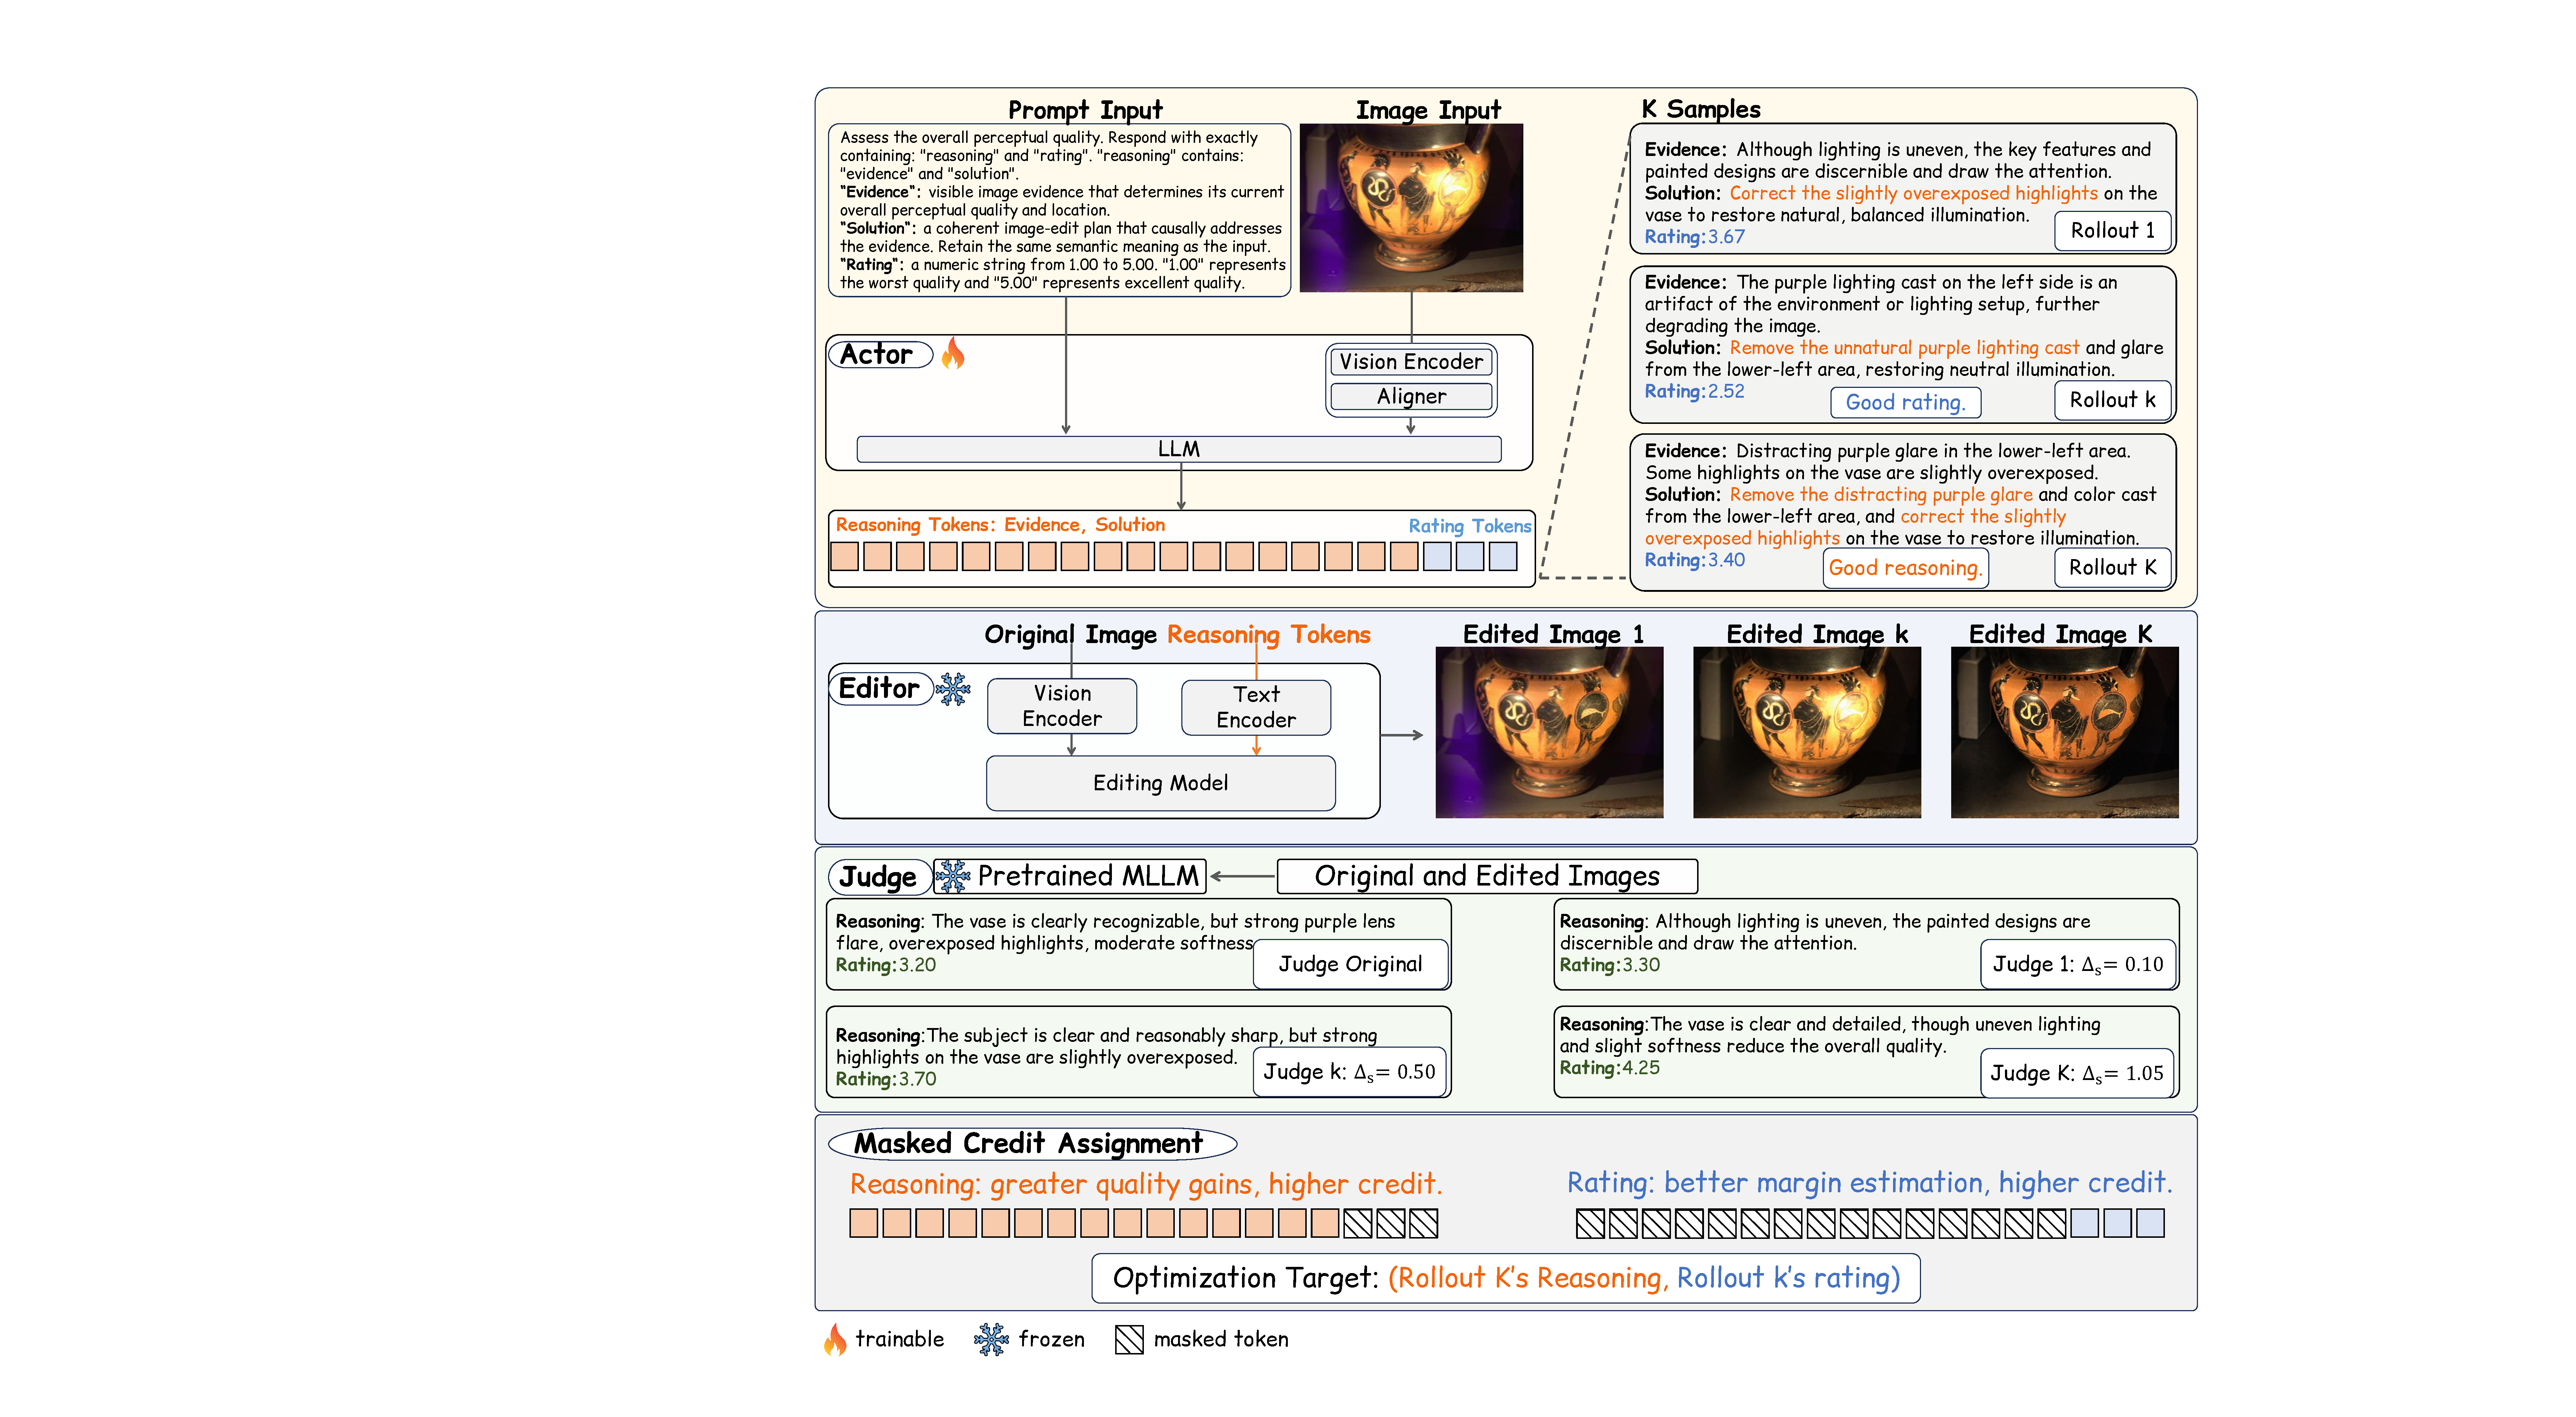
\includegraphics[
        width=\textwidth,
        height=0.68\textheight,
        keepaspectratio,
        pagebox=cropbox
    ]{Figures/figure_method.pdf}
    \caption{Overview of MR-IQA-2. Prior MLLM-based IQA produces an
    explanation and a rating without visually verifying the explanation.
    Our actor converts a quality hypothesis into multiple targeted
    low-level edits. The independent judge compares the resulting
    quality changes and returns evidence-based feedback. Only visually
    supported interventions reinforce the actor, yielding faithful
    reasoning and a deeper understanding of causal quality-limiting
    factors. Here, $\Delta s$ denotes the Judge-score change between an edited
    image and the original image, as defined in
    Eq.~\eqref{eq:judge-quality-change}.}
    \label{fig:overview}
\end{figure*}

The main contributions are summarized as follows:
\begin{itemize}
    \item We introduce fine-grained credit assignment for the reasoning--rating structure in BIQA. Masked token-specific updates decouple reasoning and rating supervision, assigning signal to its corresponding output while preserving the causal relation from reasoning to rating.

    \item We construct a verifiable supervision signal for faithful quality reasoning through visual reflection. Reasoning-conditioned editing serves as a visual intervention, while a frozen judge evaluates the observed quality change and assigns credit to the corresponding reasoning.

    \item We integrate these two mechanisms into MR-IQA-2, a modular actor-editor-judge framework that operationalizes reasoning-editing-reflection. The actor, editor, and judge can be independently instantiated or replaced for different models and downstream settings.
\end{itemize}

\section{Related Work}

\subsection{Faithful Quality Reasoning with MLLMs.}

The adoption of MLLMs has improved the interpretability of BIQA by enabling language-based image understanding and quality explanations. However, faithful quality reasoning remains a key challenge. Early methods such as DepictQA~\citep{depictqa} and Q-Instruct~\citep{q-instruct} mainly rely on supervised fine-tuning (SFT), which encourages plausible explanation patterns. Constrained by their training data, these models may overfit templated responses and exhibit limited logical coherence. Later RL-based frameworks, including Q-Insight~\citep{q-insight}, VisualQuality-R1~\citep{Visualquality-r1}, H-IQA~\citep{h-iqa}, and MR-IQA~\citep{mr-iqa}, optimize generated reasoning using rating supervision. By strengthening the model's underlying perceptual capabilities, these methods mitigate template overfitting, produce richer and more consistent reasoning, and improve rating alignment. Nevertheless, the reasoning itself is generated by the MLLM backbone without a reliable reasoning-specific supervision signal, making its faithfulness difficult to verify. Our framework instead evaluates reasoning faithfulness through visual intervention by verifying whether edits derived from the identified reasoning factors lead to observable improvements in image quality.



% \subsection{Iterative Image-Editing with MLLMs}
%
% Instruction-guided image editing has evolved from single-pass editors such as
% InstructPix2Pix~\citep{instructpix2pix} to iterative multimodal agents such as
% MIRA~\citep{mira}. The latter design has two main advantages. First, an LLM can
% expand a simple user instruction into concrete editing operations. Second, an
% LLM can also serve as an evaluator to support iterative refinement. In image
% editing, instruction following and image quality are two central objectives. A
% strong editing model should generate an output that has high visual quality and
% follows the given instruction. MIRA exemplifies this iterative MLLM-based
% editing paradigm. However, its connection to IQA is still limited by two
% differences. First, the editing instruction is usually provided by the user,
% while IQA requires the model to generate quality-improvement instructions from
% image understanding. Second, the optimization goal of image editing is to
% jointly improve instruction following and output quality, while our goal is to
% improve the model's understanding of image quality. Therefore, although our
% framework shares a similar iterative structure with MLLM-based editing, its
% instruction source, optimization target, and research objective are distinct.

\subsection{Tool-Augmented IQA Methods}

Before MLLM-based BIQA, degradation modeling and task-specific image processing were already used to derive quality cues. ARNIQA~\citep{arniqa} applies predefined degradation operators to construct contrastive views and learn distortion-aware representations. More recently, Zoom-IQA~\citep{zoom-iqa} introduces region-aware zooming for detail inspection. Tool-IQA~\citep{tool-iqa} further employs a magnifier and a gamma corrector to provide additional visual evidence for quality rating. Although these tools enable richer and more localized inspection, the resulting reasoning is still evaluated mainly through rating performance. Rather than enriching the visual evidence during reasoning for rating optimization, our design provides direct supervision for the faithfulness of quality reasoning.

\section{Methods}
\label{sec:methods}

\subsection{MR-IQA-2 Framework Overview}
In this work, we propose MR-IQA-2 (Figure~\ref{fig:overview}), an actor-editor-judge framework for faithful IQA. MR-IQA-2 makes quality reasoning verifiable rather than assessing it solely through rating performance. The actor is a general MLLM-based BIQA model that produces interpretable quality reasoning and a rating. A frozen editor, initialized from an image-editing diffusion model, applies edits conditioned on the reasoning. A frozen MLLM judge then evaluates the quality change between the original and edited images. The observed change provides a reasoning-specific supervision signal for the actor. The following sections introduce (1) the interaction among the actor, editor, and judge, (2) fine-grained credit assignment, and (3) the training optimization procedure.

\subsection{Actor-Editor-Judge Trajectory}
\label{sec:actor-editor-judge-trajectory}
This section describes the interaction flow among the Actor, Editor, and Judge.
For a local batch of $N$ images, $i\in\{1,\ldots,N\}$ indexes an image, $K$
denotes the number of Actor samples per image, and $k\in\{1,\ldots,K\}$ indexes
one sample.
Within each training trajectory, superscript $b\in\{0,1\}$ denotes the
original-image and post-editing stages, respectively. \\
\textbf{Actor} receives an original image $I_i^0$ and uses a prompt $P_A$ to
generate quality reasoning and a rating:
\begin{equation}
    a_{i,k}^0
    =
    \left(r_{i,k}^0,q_{i,k}^0\right)
    \sim
    \pi_{\mathrm{old}}\!\left(\cdot\mid I_i^0,P_A\right),
    \label{eq:actor-initial-rollout}
\end{equation}
where $\pi_{\mathrm{old}}$ denotes the original Actor policy used to generate
the rollouts, and $r_{i,k}^0$ and $q_{i,k}^0$ denote reasoning and rating. \\
\textbf{Editor} corrects the quality factors identified by the Actor:
\begin{equation}
    I_{i,k}^1
    =
    E_{\phi_E}\!\left(I_i^0,r_{i,k}^0;P_E\right),
    \qquad \phi_E\ \text{fixed}.
    \label{eq:editor-intervention}
\end{equation}
where $P_E$ is a fixed editing prompt template and $I_{i,k}^1$ is the edited
output.\\
\textbf{Judge} independently rates the original and edited images:
\begin{equation}
    s_i^0
        =J_{\phi_J}\!\left(I_i^0\right),
    \qquad
    s_{i,k}^1
        =J_{\phi_J}\!\left(I_{i,k}^1\right).
    \label{eq:judge-evaluation}
\end{equation}
The resulting trajectory is
\begin{equation}
    \mathcal{T}_{i,k}
    =
    \left(
    I_i^0,a_{i,k}^0,I_{i,k}^1,s_i^0,s_{i,k}^1
    \right).
    \label{eq:actor-editor-judge-trajectory}
\end{equation}
The Judge-observed quality change is
\begin{equation}
    \Delta s_{i,k}=s_{i,k}^1-s_i^0.
    \label{eq:judge-quality-change}
\end{equation}

\subsection{Fine-Grained Credit Assignment}
\paragraph{Motivation.}
As discussed in the Introduction, higher rating accuracy alone does not
guarantee faithful reasoning. Moreover, assigning a shared reward to reasoning
and rating obscures the source of supervision. We therefore define separate
rewards for reasoning, rating, and format, and use each reward to update its
corresponding output tokens.

\paragraph{Reasoning reward.}
For each image, the Actor samples $K$ reasoning--rating outputs indexed by
$k$. Each reasoning proposal is evaluated with the frozen Editor and
Judge. The editing prompt restricts interventions to low-level quality
attributes while preserving image content. We measure reasoning faithfulness
by the resulting Judge-score improvement:
\begin{equation}
    R_{i,k}^{\mathrm{reasoning}}
    =
    \Delta s_{i,k}.
    \label{eq:reasoning-reward}
\end{equation}
Under these controlled conditions, reasoning that produces a larger quality
improvement receives a higher reward.

\paragraph{Rating reward.}
Following MR-IQA~\citep{mr-iqa}, we supervise rating through relative quality
margins. Let $y_i$ be the human mean opinion score (MOS). For another image
$j\ne i$ in the same batch, the scale-controlled margin error is
\begin{equation}
    z_{i,k,j}^{\mathrm{rating}}
    =
    \frac{
    \left(q_{i,k}^0-\frac{1}{K}\sum_{k'=1}^{K}q_{j,k'}^0\right)
    -
    \left(y_i-y_j\right)
    }{\tau_{ij}},
    \label{eq:rating-margin-error}
\end{equation}
where $\tau_{ij}>0$ controls the margin-error scale. Using the L2 estimator, we
average the $N-1$ pairwise rewards:
\begin{equation}
    R_{i,k}^{\mathrm{rating}}
    =
    \frac{1}{N-1}
    \sum_{\substack{j=1\\j\ne i}}^{N}
    \mathrm{e}^{-\frac{1}{2}\left(z_{i,k,j}^{\mathrm{rating}}\right)^2}.
    \label{eq:rating-reward}
\end{equation}

\paragraph{Format reward.}
The Actor output must be a valid JSON object containing the ordered fields
\textbf{reasoning} and \textbf{rating}. Let $\mathcal{F}$ denote this output
contract. The format reward is
\begin{equation}
    R_{i,k}^{\mathrm{format}}
    =
    \mathbf{1}\!\left[a_{i,k}^0\in\mathcal{F}\right].
    \label{eq:format-reward}
\end{equation}

\paragraph{Masked credit assignment.}
Let $c$ index a supervision type. For token $t$, $\chi_{i,k,t}^c$ is its binary
mask, and $\Omega_{i,k}^c$ is the selected token set:
\begin{equation}
\begin{aligned}
    \mathcal{C}
        &=
        \{\mathrm{reasoning},\mathrm{rating},\mathrm{format}\},\\
    \Omega_{i,k}^c
        &=
        \left\{t\,\middle|\,\chi_{i,k,t}^c=1\right\},
        \qquad c\in\mathcal{C}.
\end{aligned}
    \label{eq:credit-token-set}
\end{equation}
Each reward is normalized independently within the $K$ samples of image $i$:
\begin{equation}
    A_{i,k}^c
        =\frac{R_{i,k}^c-\mu_i^c}{\sigma_i^c+\epsilon_A}.
    \label{eq:reward-wise-advantage}
\end{equation}
Here, $\mu_i^c$ and $\sigma_i^c$ denote the corresponding group mean and sample
standard deviation. The masked advantage for each supervision type is
\begin{equation}
    \widetilde A_{i,k,t}^c
    =
    \chi_{i,k,t}^c A_{i,k}^c.
    \label{eq:token-level-credit}
\end{equation}
Thus, reasoning and rating rewards update only their corresponding fields,
whereas the format reward applies to the complete output.

\subsection{Masked Credit with GRPO}
We optimize the Actor with Group Relative Policy Optimization
(GRPO)~\citep{shao2024deepseekmath}. Let $\mathcal{I}_c$ contain the valid
sampled outputs for supervision type $c$. Using the masked advantage in
Eq.~\eqref{eq:token-level-credit}, the masked GRPO loss is
\begin{equation}
\begin{aligned}
    \mathcal{L}_{\mathrm{GRPO}}(\theta)
        &=-\sum_{c\in\mathcal{C}}\frac{1}{|\mathcal{I}_c|}
        \sum_{(i,k)\in\mathcal{I}_c}
        \frac{1}{|\Omega_{i,k}^c|}
        \sum_{t\in\Omega_{i,k}^c}\omega_{i,k,t}\\
        &\quad{}\times
        \min\left(
            \rho_{i,k,t}\widetilde A_{i,k,t}^c,
            \rho_{i,k,t}^{\mathrm{clip}}\widetilde A_{i,k,t}^c
        \right).
\end{aligned}
    \label{eq:masked-grpo-loss}
\end{equation}
Here, $\rho_{i,k,t}$ is the likelihood ratio between the current Actor
$\pi_\theta$ and the rollout policy $\pi_{\mathrm{old}}$.
$\rho_{i,k,t}^{\mathrm{clip}}$ clips this ratio to
$[1-\epsilon_{\mathrm{low}},1+\epsilon_{\mathrm{high}}]$.
$\omega_{i,k,t}$ corrects the token-level mismatch between the rollout
distribution and $\pi_{\mathrm{old}}$ and is capped by $\omega_{\max}$.

\begin{table*}[!t]
\centering
{\small
\setlength{\tabcolsep}{2pt}
\begin{tabular}{@{}l cc cc cc cc cc cc cc@{}}
\toprule
& \multicolumn{6}{c}{Authentic} & \multicolumn{2}{c}{AI-generated} &
\multicolumn{4}{c}{Synthetic} & \multicolumn{2}{c}{Average} \\
\cmidrule(lr){2-7} \cmidrule(lr){8-9} \cmidrule(lr){10-13}
\cmidrule(lr){14-15}
& \multicolumn{2}{c}{KonIQ} & \multicolumn{2}{c}{SPAQ} &
\multicolumn{2}{c}{LIVE-W} & \multicolumn{2}{c}{AGIQA-3K} &
\multicolumn{2}{c}{KADID-10k} & \multicolumn{2}{c}{CSIQ} &
\multicolumn{2}{c}{Avg.} \\
\cmidrule(lr){2-3} \cmidrule(lr){4-5} \cmidrule(lr){6-7}
\cmidrule(lr){8-9} \cmidrule(lr){10-11} \cmidrule(lr){12-13}
\cmidrule(lr){14-15}
Method & PLCC & SRCC & PLCC & SRCC & PLCC & SRCC & PLCC & SRCC &
PLCC & SRCC & PLCC & SRCC & PLCC & SRCC \\
\midrule
\multicolumn{15}{@{}l}{\textit{Hand-crafted}} \\
NIQE~\citeyearpar{NIQE}
& 0.533 & 0.530 & 0.679 & 0.664 & 0.493 & 0.449 & 0.560 & 0.533
& 0.468 & 0.405 & 0.718 & 0.628 & 0.575 & 0.535 \\
BRISQUE~\citeyearpar{BRISQUE}
& 0.225 & 0.226 & 0.490 & 0.406 & 0.361 & 0.313 & 0.541 & 0.497
& 0.429 & 0.356 & 0.740 & 0.556 & 0.464 & 0.392 \\
\midrule
\multicolumn{15}{@{}l}{\textit{Deep-learning-based}} \\
NIMA~\citeyearpar{nima}
& 0.896 & 0.859 & 0.838 & 0.856 & 0.814 & 0.771 & 0.715 & 0.654
& 0.532 & 0.535 & 0.695 & 0.649 & 0.748 & 0.721 \\
DBCNN~\citeyearpar{dbcnn}
& 0.884 & 0.875 & 0.812 & 0.806 & 0.773 & 0.730 & 0.641 & 0.648
& 0.497 & 0.484 & 0.586 & 0.572 & 0.699 & 0.686 \\
MUSIQ~\citeyearpar{musiq}
& 0.924 & 0.929 & 0.868 & 0.863 & 0.789 & 0.830 & 0.722 & 0.630
& 0.575 & 0.556 & 0.771 & 0.710 & 0.775 & 0.753 \\
MANIQA~\citeyearpar{yang2022maniqa}
& 0.849 & 0.834 & 0.768 & 0.758 & 0.849 & 0.832 & 0.723 & 0.636
& 0.499 & 0.465 & 0.623 & 0.627 & 0.719 & 0.692 \\
CLIP-IQA+~\citeyearpar{wang2023exploring}
& 0.909 & 0.895 & 0.866 & 0.864 & 0.832 & 0.805 & 0.736 & 0.685
& 0.653 & 0.654 & 0.772 & 0.719 & 0.795 & 0.770 \\
\midrule
\multicolumn{15}{@{}l}{\textit{MLLM-based: SFT training}} \\
C2Score~\citeyearpar{zhu2024adaptive}
& 0.923 & 0.910 & 0.867 & 0.860 & 0.786 & 0.772 & 0.777 & 0.671
& 0.500 & 0.453 & 0.735 & 0.705 & 0.765 & 0.729 \\
Q-Align~\citeyearpar{q-align}
& 0.941 & \textcolor{secondbestblue}{0.940}
& 0.886 & 0.887 & 0.853 & 0.860 & 0.772 & 0.735
& 0.674 & 0.684 & 0.671 & 0.737 & 0.800 & 0.807 \\
DeQA~\citeyearpar{deqa}
& \textcolor{bestred}{0.953} & \textcolor{bestred}{0.941}
& 0.895 & 0.896 & 0.892 & \textcolor{secondbestblue}{0.879}
& 0.809 & 0.729
& 0.694 & 0.687 & 0.787 & 0.744
& \textcolor{secondbestblue}{0.838} & 0.813 \\
\midrule
\multicolumn{15}{@{}l}{\textit{MLLM-based: RL training}} \\
Q-Insight~\citeyearpar{q-insight}
& 0.918 & 0.895 & \textcolor{bestred}{0.903}
& \textcolor{bestred}{0.903} & 0.870 & 0.839
& \textcolor{secondbestblue}{0.816} & \textcolor{secondbestblue}{0.766}
& \textcolor{bestred}{0.702} & \textcolor{bestred}{0.702}
& 0.685 & 0.640 & 0.816 & 0.791 \\
VQ-R1~\citeyearpar{Visualquality-r1}
& 0.886 & 0.919 & 0.867 & 0.887 & 0.817 & 0.869 & 0.744 & 0.718
& 0.635 & 0.640 & 0.709 & 0.721 & 0.776 & 0.792 \\
MR-IQA~\citeyearpar{mr-iqa}
& 0.949 & 0.931
& 0.892 & 0.897 & \textcolor{bestred}{0.899}
& \textcolor{bestred}{0.883} & 0.804 & 0.732 & 0.672 & 0.683
& 0.767 & 0.732 & 0.831 & 0.810 \\
\midrule
\multicolumn{15}{@{}l}{\textit{MLLM-based: Tool-augmented training}} \\
Zoom-IQA$^{\dagger}$~\citeyearpar{zoom-iqa}
& 0.938 & 0.922
& \textcolor{secondbestblue}{0.902} & \textcolor{secondbestblue}{0.900}
& 0.887 & 0.870
& \textcolor{secondbestblue}{0.816} & 0.765
& \textcolor{secondbestblue}{0.701} & \textcolor{secondbestblue}{0.700}
& \textcolor{secondbestblue}{0.797} & \textcolor{secondbestblue}{0.754}
& \textcolor{bestred}{0.840} & \textcolor{bestred}{0.819} \\
\textbf{MR-IQA-2 (Ours)}
& \textcolor{secondbestblue}{0.952} & 0.938
& 0.901 & 0.898
& \textcolor{secondbestblue}{0.897} & 0.877
& \textcolor{secondbestblue}{0.816} & 0.747
& 0.661 & 0.668 & 0.771 & 0.746 & 0.833 & 0.812 \\
\textbf{MR-IQA-2$^{*}$ (Ours)}
& 0.925 & 0.904
& 0.901 & \textcolor{secondbestblue}{0.900}
& 0.881 & 0.847
& \textcolor{bestred}{0.826} & \textcolor{bestred}{0.768}
& 0.665 & 0.676
& \textcolor{bestred}{0.840} & \textcolor{bestred}{0.801}
& \textcolor{bestred}{0.840} & \textcolor{secondbestblue}{0.816} \\
\bottomrule
\end{tabular}
}
\caption{\textbf{Rating performance comparison.} Each dataset reports
PLCC$\uparrow$ and SRCC$\uparrow$ between predicted and ground-truth ratings.
\textcolor{bestred}{Red} and \textcolor{secondbestblue}{blue} denote the best
and second-best results, respectively. Baseline entries use reported results, except that VQ-R1 is reproduced with
Qwen3-VL-2B~\citep{qwen3vl} because its original results were obtained under a
different training protocol. Both MR-IQA-2 variants use Qwen3.5-4B;
MR-IQA-2$^{*}$ freezes the vision encoder and aligner during training.
Zoom-IQA$^{\dagger}$ uses additional annotations and combines
SFT with RL; all other trainable methods use the same KonIQ training split.}
\label{tab:main}

{\small
\setlength{\tabcolsep}{6pt}
\begin{tabular*}{\textwidth}{@{\extracolsep{\fill}}l|rr|rr|c@{}}
\toprule
& \multicolumn{2}{c|}{\textbf{Pretrained Judge}}
& \multicolumn{2}{c|}{\textbf{Q-Insight as Judge}}
& \multicolumn{1}{c}{\textbf{GPT-5.6 Sol as Judge (\%)}} \\
\midrule
\diagbox[width=10.5em,height=2.8\baselineskip]{\textbf{Actor}}{\textbf{Editor}}
& \multicolumn{1}{c}{\textbf{FLUX.2 [klein]}}
& \multicolumn{1}{c|}{\textbf{Mage-Flow}}
& \multicolumn{1}{c}{\textbf{FLUX.2 [klein]}}
& \multicolumn{1}{c|}{\textbf{Mage-Flow}}
& \multicolumn{1}{c}{\textbf{FLUX.2 [klein]}} \\
\midrule
Qwen3.5-4B (Baseline) & $-0.137$ & $-0.144$ & $-0.130$ & $-0.080$ & $4.19\%$ \\
Q-Insight & $+0.213$ & $+0.142$ & $+0.138$ & $+0.139$ & $14.41\%$ \\
\textbf{MR-IQA-2 (Ours)} & $\mathbf{+0.789}$ & $\mathbf{+0.468}$
& $\mathbf{+0.561}$ & $\mathbf{+0.376}$ & $\mathbf{81.40\%}$ \\
\bottomrule
\end{tabular*}
}
\caption{\textbf{Reasoning performance validation.} The first four columns
report mean quality gain $\Delta s$ (higher is better;
Eq.~\eqref{eq:judge-quality-change}); GPT-5.6 Sol uses 3-Alternative Forced Choice (3AFC). We compare
the Qwen3.5-4B baseline~\citep{qwen35}, Q-Insight~\citep{q-insight}, and
MR-IQA-2 (ours). The 4B four-step LoRA Editors are FLUX.2
[klein]~\citep{flux2} and Mage-Flow~\citep{zhang2026mageflow}. Judges are our
pretrained Qwen3.5-4B Judge~\citep{qwen35}, Q-Insight~\citep{q-insight}, and
GPT-5.6 Sol~\citep{openai2026gpt56sol}. Evaluation uses a fixed
5,866-image subset formed by randomly selecting 1,000 images from each test set,
except CSIQ, for which all 866 images are used.}
\label{tab:cross-tool-reasoning}
\end{table*}

\section{Experiments}
\label{sec:experiments}

\subsection{Experimental Settings}
\label{sec:experimental-settings}

\paragraph{Datasets.}
We train all controlled models on the training subset of
the KonIQ-10k split~\citep{koniq}, which contains $7{,}046$
in-the-wild images at $512{\times}384$ resolution. We evaluate on the
KonIQ-10k test split (2,010 images) as the in-distribution authentic benchmark.
For out-of-distribution (OOD) evaluation, we use the authentic distortion
datasets SPAQ (11,125 images)~\citep{spaq} and LIVE In the Wild
(LIVE-W; 1,162 images)~\citep{live-w}, as well as the AI-generated image
quality dataset AGIQA-3K (2,982 images)~\citep{agiqa}. We further include the
synthetic distortion datasets KADID-10k (10,125 images)~\citep{kadid} and CSIQ
(866 images)~\citep{csiq}.

\paragraph{Model Backbones.}
The \textbf{Actor} is initialized from Qwen3.5-4B~\citep{qwen35}, selected for
its balance of visual reasoning and efficiency. The \textbf{Editor} uses
FLUX.2 [klein] 4B~\citep{flux2} with a four-step LoRA for fast and efficient
editing. It runs in BF16 with classifier-free guidance $1.0$ and sigma schedule
$[1.0,0.75,0.5,0.25]$. The \textbf{Judge} uses a Qwen3.5-4B checkpoint trained
for 5 epochs on KonIQ-7k with rating supervision, selected for the same balance
of visual reasoning and efficiency. On a single NVIDIA RTX A6000, the Editor's
mean inference time is $0.902$\,s per image, while Judge inference takes $0.800$\,s per image.
During GRPO optimization, only the Actor is updated; the frozen Editor and
Judge provide offline supervision and receive no gradients.

\paragraph{Implementation Details.}
We train Qwen3.5-4B~\citep{qwen35} for five epochs on eight 48-GB NVIDIA RTX
A6000 GPUs. Each rank processes $N=6$ images and samples $K=6$ completions per
image. The maximum completion length is 192 tokens. We use
AdamW~\citep{adam} with
$(\beta_1,\beta_2)=(0.9,0.95)$,
$\epsilon_{\mathrm{Adam}}=10^{-8}$, a learning rate of $10^{-6}$, weight decay
of $0.1$, cosine scheduling without warmup, and gradient-norm clipping at
$1.0$. We use symmetric policy clipping with
$(\epsilon_{\mathrm{low}},\epsilon_{\mathrm{high}})=(0.20,0.20)$, no hard
clipping of advantages, and token-level importance-ratio truncation at
$\omega_{\max}=2$. Rollouts use
temperature $0.7$, top-$p$ $1.0$, top-$k$ $20$, and a presence penalty of
$1.5$. Actor-only training takes approximately $2$ hours per epoch. For the
full MR-IQA-2 framework, four GPUs are allocated to Actor training and four to
Editor--Judge inference, increasing the per-epoch time to approximately $12$
hours.

\subsection{Rating Performance}
\label{sec:rating-performance}

\paragraph{Compared methods.}
Table~\ref{tab:main} compares MR-IQA-2 with representative BIQA methods across
six benchmarks. The hand-crafted group includes NIQE~\citep{NIQE} and
BRISQUE~\citep{BRISQUE}. Deep-learning-based methods include
NIMA~\citep{nima}, DBCNN~\citep{dbcnn}, MUSIQ~\citep{musiq},
MANIQA~\citep{yang2022maniqa}, and CLIP-IQA+~\citep{wang2023exploring}.
Among MLLM-based methods, SFT approaches include
C2Score~\citep{zhu2024adaptive}, Q-Align~\citep{q-align}, and
DeQA~\citep{deqa}, while RL approaches include Q-Insight~\citep{q-insight},
VQ-R1~\citep{Visualquality-r1}, and MR-IQA~\citep{mr-iqa}. We further compare
with the tool-augmented RL method Zoom-IQA~\citep{zoom-iqa}. For MR-IQA-2, we
report an active-vision checkpoint and a frozen-vision variant, denoted by
$^{*}$.

\paragraph{Efficiency and performance.}
MR-IQA-2 is designed primarily to improve reasoning faithfulness rather than
maximize rating. Nevertheless, it achieves competitive rating
performance. \textbf{(1)} Zoom-IQA~\citep{zoom-iqa} uses a two-stage SFT--RL
pipeline with additional annotations, whereas MR-IQA-2 uses only RL training without additional data requirement. The frozen-vision variant
reaches an average PLCC/SRCC of 0.840/0.816, comparable to Zoom-IQA's
0.840/0.819. \textbf{(2)} We further observe that freezing the vision encoder
and aligner is particularly effective on AI-generated and synthetic datasets.
The frozen variant achieves the best CSIQ PLCC/SRCC of 0.840/0.801, whereas
active visual training yields its main gains on the authentic datasets.


\subsection{Faithful Reasoning Performance}
\label{sec:faithful-reasoning-performance}
\paragraph{Quality Gain as a Proxy for Reasoning Faithfulness.}
Prior work, including Q-Insight~\citep{q-insight} and
VisualQuality-R1~\citep{Visualquality-r1}, typically evaluates reasoning through human inspection of a small number of examples or indirectly through improvements in rating performance. These practices lack a unified evaluation criterion. In this work, we instead use the image-quality gain produced by reasoning-guided editing as the evaluation criterion (Eq.~(\ref{eq:reasoning-reward})), rather than rating performance. We assume that faithful reasoning should identify quality-limiting factors whose correction improves the given image.
\paragraph{Cross-editor/judge stability.}
Table~\ref{tab:cross-tool-reasoning} examines whether the Actor overfits to the
frozen Editor--Judge during training. We first replace the FLUX.2 [klein] Editor~\citep{flux2} with
Mage-Flow~\citep{zhang2026mageflow}. MR-IQA-2 retains larger quality gains than
the competing Actors, indicating that its reasoning is not specific to a single
Editor. We then replace the pretrained Judge with
Q-Insight~\citep{q-insight} and GPT-5.6 Sol~\citep{openai2026gpt56sol}. These
alternative Judges preserve the direction of the measured gains. These results indicate that the Actor learns
generalizable quality knowledge rather than exploiting idiosyncrasies of the
training-time Editor or Judge.

\paragraph{Quality and behavior analysis.}
Additional analyses (in Appendix Figure 4) provide four observations. (a) Across all datasets,
lower-quality images obtain larger quality gains. (b) Changes in sharpness are
strongly associated with Judge preference. (c) Higher-quality images tend to
remain closer to their originals after editing. (d) Training shifts the Actor
toward quality-relevant reasoning tokens.

\subsection{Ablation Study}
\label{sec:ablation-study}

\paragraph{Evaluation.}
Table~\ref{tab:credit-ablation-rating} reports ablations on rating alignment and
reasoning-guided quality improvement. Rating-only training already achieves
competitive rating alignment, with an average PLCC/SRCC of $0.836/0.815$. However,
its mean quality gain is $-0.260$, below the baseline result of $-0.161$.
Rating performance alone therefore does not guarantee faithful reasoning.
Adding the reasoning reward changes the quality gain from $-0.260$ to
$+0.838$. The credit mask further increases the gain to $+0.917$, although its
additional benefit is modest after rating alignment has stabilized.

The credit mask is more beneficial early in training. At step 30 on the
200-image validation set, it reaches a PLCC/SRCC of $0.745/0.772$, compared
with $0.667/0.617$ without the credit mask and $0.616/0.610$ for the baseline.
Its quality gain is lower at this stage, at $0.255$ versus $0.387$ without the
credit mask. This suggests that the credit mask accelerates rating convergence
but may temporarily limit reasoning improvement. Once rating alignment
stabilizes, its benefit becomes smaller. This behavior warrants further study
of the imbalance between rating and reasoning rewards.

\begin{table*}[t]
\centering
{\small
\setlength{\tabcolsep}{2pt}
\begin{tabular}{@{}l cc cc cc cc cc cc cc@{}}
\toprule
\multicolumn{15}{@{}l}{\textit{Rating alignment}} \\
& \multicolumn{6}{c}{Authentic} & \multicolumn{2}{c}{AI-generated} &
\multicolumn{4}{c}{Synthetic} & \multicolumn{2}{c}{Average} \\
\cmidrule(lr){2-7} \cmidrule(lr){8-9} \cmidrule(lr){10-13}
\cmidrule(lr){14-15}
& \multicolumn{2}{c}{KonIQ} & \multicolumn{2}{c}{SPAQ} &
\multicolumn{2}{c}{LIVE-W} & \multicolumn{2}{c}{AGIQA-3K} &
\multicolumn{2}{c}{KADID-10k} & \multicolumn{2}{c}{CSIQ} &
\multicolumn{2}{c}{Avg.} \\
\cmidrule(lr){2-3} \cmidrule(lr){4-5} \cmidrule(lr){6-7}
\cmidrule(lr){8-9} \cmidrule(lr){10-11} \cmidrule(lr){12-13}
\cmidrule(lr){14-15}
\textbf{Method} & PLCC & SRCC & PLCC & SRCC & PLCC & SRCC & PLCC & SRCC &
PLCC & SRCC & PLCC & SRCC & PLCC & SRCC \\
\midrule
Baseline
& 0.553 & 0.583 & 0.750 & 0.743 & 0.592 & 0.564
& 0.679 & 0.655 & 0.660 & 0.669 & 0.681 & 0.657 & 0.652 & 0.645 \\
Rating-only
& 0.952 & 0.938 & \textbf{0.901} & \textbf{0.899} & 0.896 & 0.875
& 0.808 & 0.740 & \textbf{0.669} & \textbf{0.676}
& \textbf{0.789} & \textbf{0.764} & \textbf{0.836} & \textbf{0.815} \\
Without credit mask
& \textbf{0.952} & \textbf{0.938} & 0.901 & 0.898
& \textbf{0.897} & \textbf{0.877}
& \textbf{0.816} & \textbf{0.747} & 0.661 & 0.668 & 0.771 & 0.746
& 0.833 & 0.812 \\
Credit mask
& 0.946 & 0.931 & 0.894 & 0.893 & 0.892 & 0.868
& 0.805 & 0.719 & 0.641 & 0.650 & 0.758 & 0.727 & 0.822 & 0.798 \\
% Credit mask + SegKL
% & 0.951 & 0.938 & 0.896 & 0.895 & 0.904 & 0.880
% & 0.801 & 0.731 & 0.654 & 0.664 & 0.784 & 0.758 & 0.831 & 0.811 \\
\midrule
\multicolumn{15}{@{}l}{\textit{Subset quality gains}} \\
\textbf{Method}
& \multicolumn{3}{c}{\textbf{Original mean}}
& \multicolumn{4}{c}{\textbf{Edited mean}}
& \multicolumn{3}{c}{\textbf{Mean gain}}
& \multicolumn{4}{c}{\textbf{Positive gain (\%)}} \\
\cmidrule(lr){2-4} \cmidrule(lr){5-8} \cmidrule(lr){9-11}
\cmidrule(lr){12-15}
Baseline
& \multicolumn{3}{c}{$2.841$}
& \multicolumn{4}{c}{$2.680$}
& \multicolumn{3}{c}{$-0.161$}
& \multicolumn{4}{c}{$40.66\%$} \\
Rating-only
& \multicolumn{3}{c}{$2.841$}
& \multicolumn{4}{c}{$2.581$}
& \multicolumn{3}{c}{$-0.260$}
& \multicolumn{4}{c}{$30.67\%$} \\
Without credit mask
& \multicolumn{3}{c}{$2.841$}
& \multicolumn{4}{c}{$3.679$}
& \multicolumn{3}{c}{$+0.838$}
& \multicolumn{4}{c}{$96.95\%$} \\
\textbf{Credit mask}
& \multicolumn{3}{c}{$2.844$}
& \multicolumn{4}{c}{$\mathbf{3.761}$}
& \multicolumn{3}{c}{$\mathbf{+0.917}$}
& \multicolumn{4}{c}{$\mathbf{97.71\%}$} \\
% Credit mask + SegKL
% & \multicolumn{3}{c}{$2.841$}
% & \multicolumn{4}{c}{$3.630$}
% & \multicolumn{3}{c}{$+0.789$}
% & \multicolumn{4}{c}{$95.04\%$} \\
\bottomrule
\end{tabular}
}
\caption{\textbf{Rating and quality-gain ablations.} The upper panel reports
PLCC/SRCC on the complete test sets and their six-dataset macro average. The
lower panel reports Judge scores before and after reasoning-guided editing on
the same 5,866-image subset used in Table~\ref{tab:cross-tool-reasoning}. Bold
marks the best result before rounding within each panel.}
\label{tab:credit-ablation-rating}
\end{table*}

\begin{figure*}[!t]
\centering
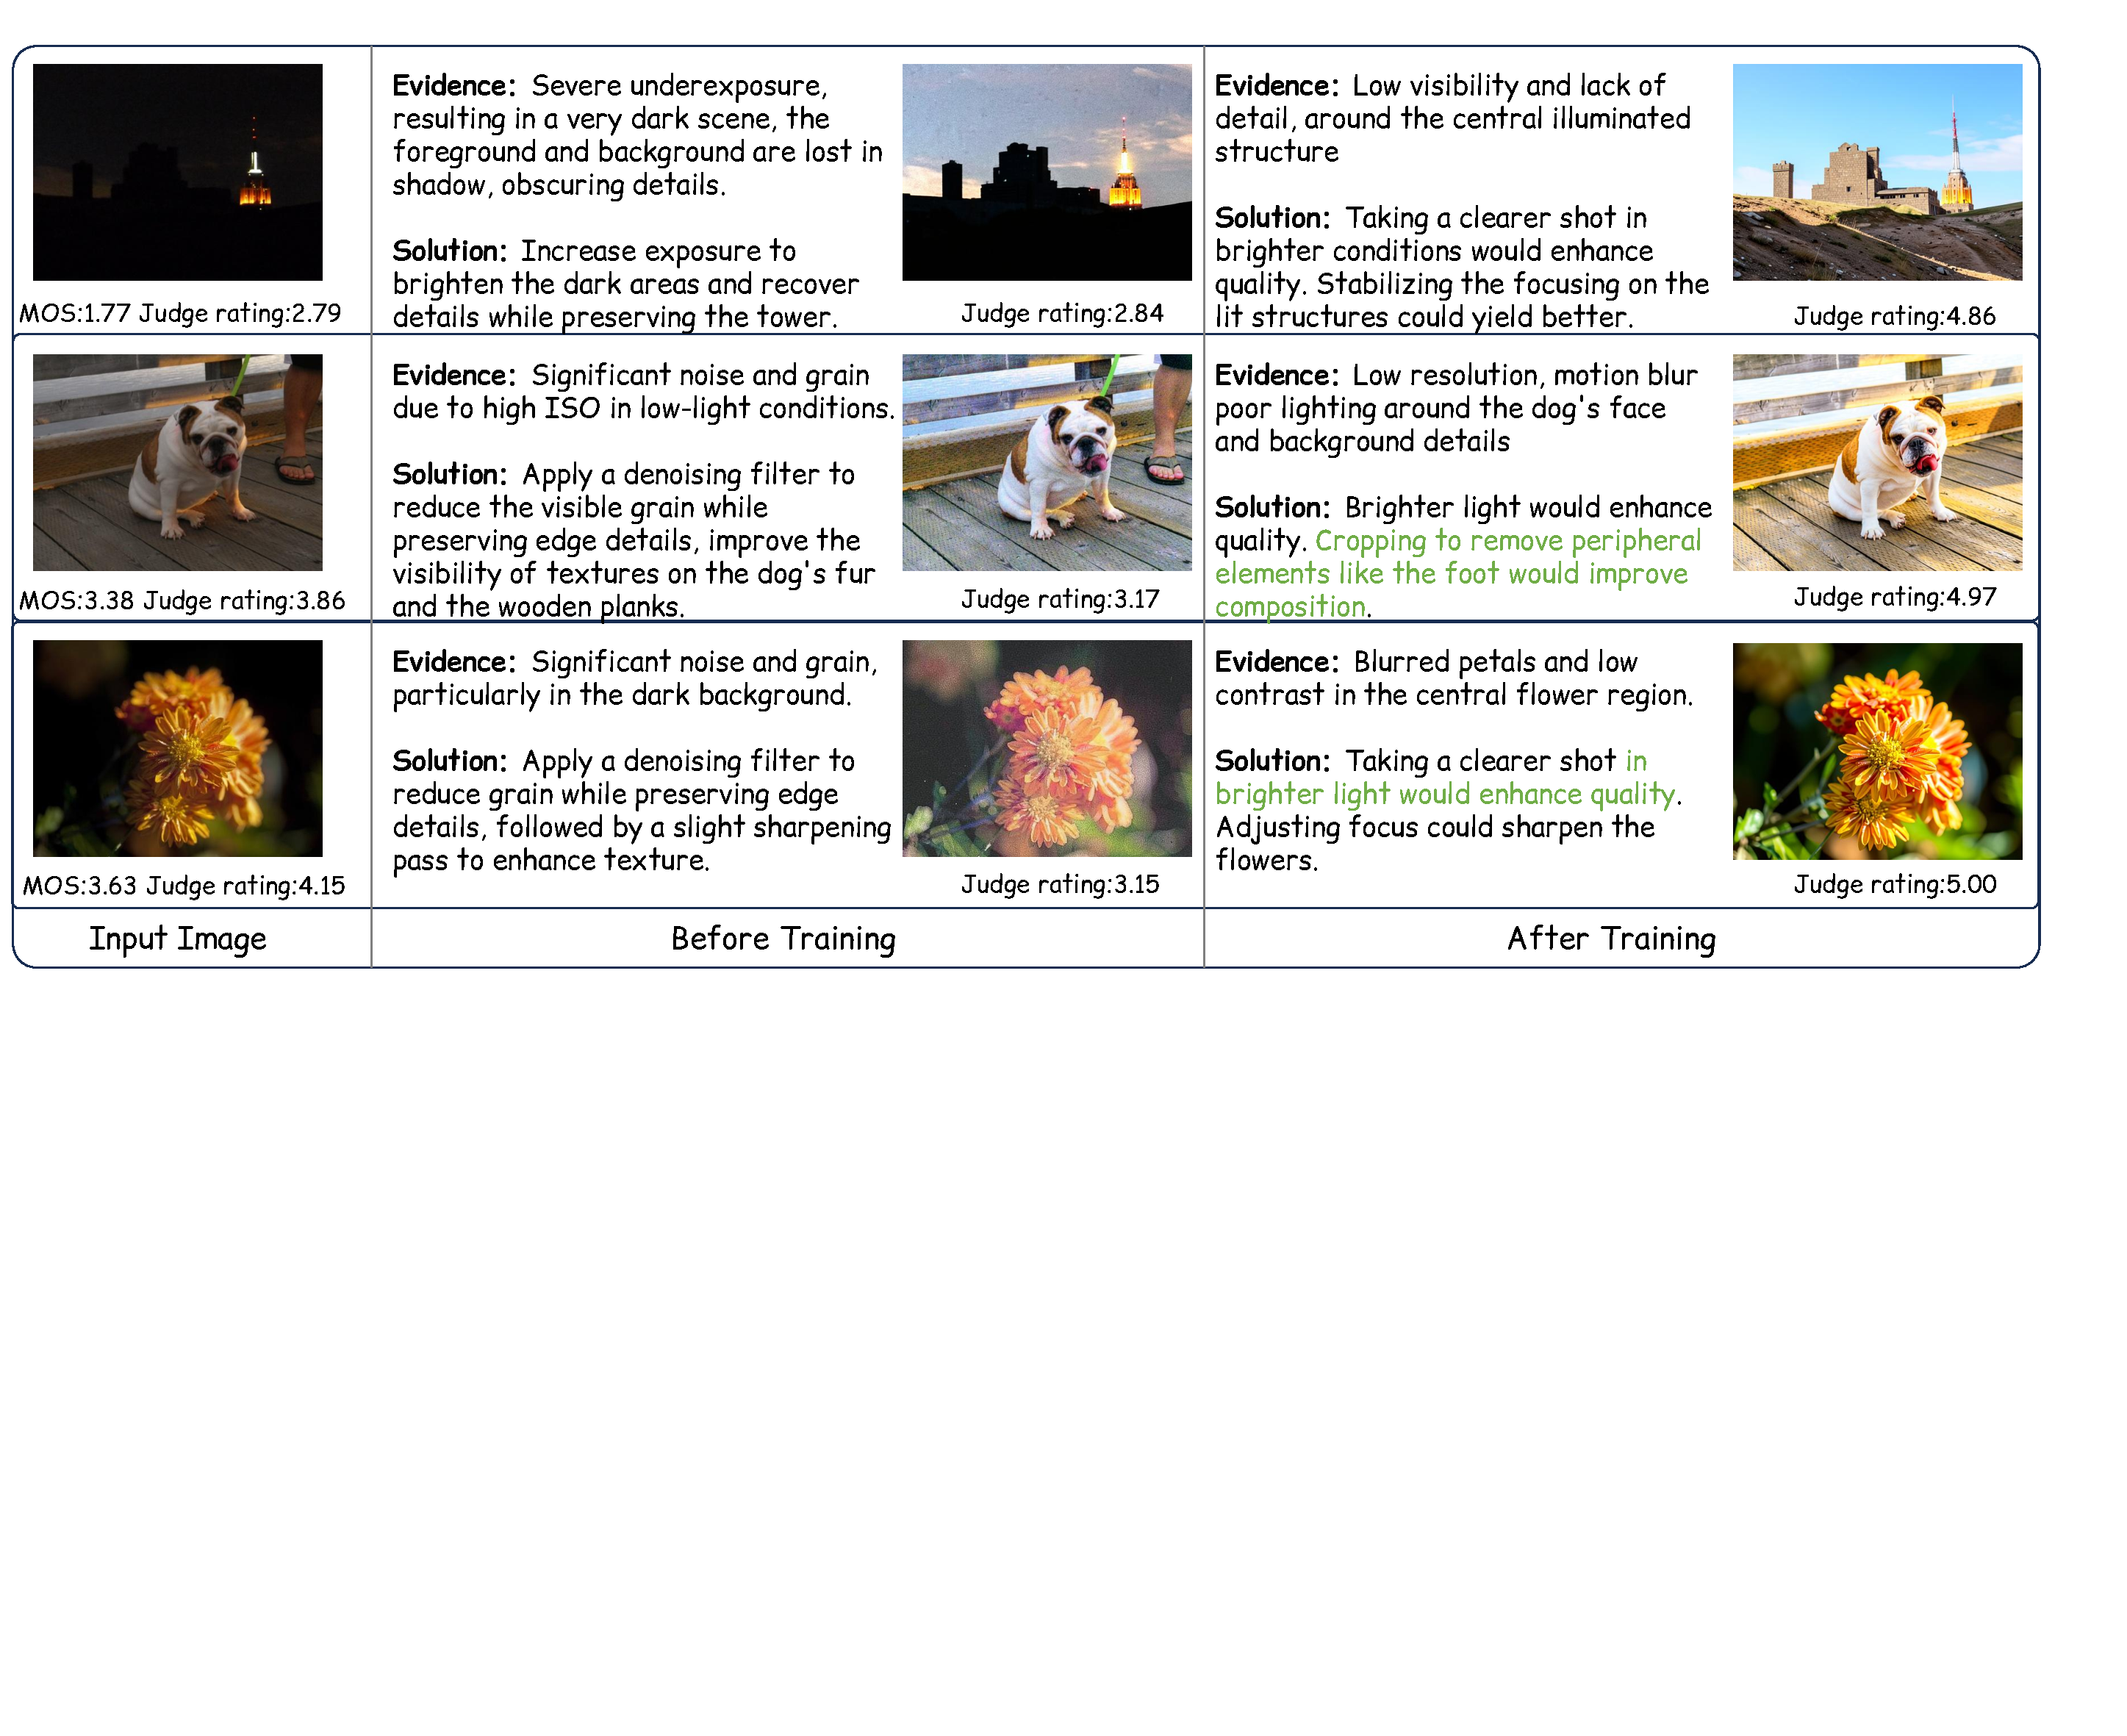
\includegraphics[width=\textwidth]{Figures/figure_case_study.pdf}
\caption{\textbf{Qualitative comparison before and after training.} Each row
shows the input image and the Actor's reasoning-guided edits before and after
training. Post-training reasoning yields more effective interventions and
larger Judge-rated quality gains. Green text highlights additional quality
factors identified after training.}
\label{fig:case-study}
\end{figure*}

\subsection{Case Study}
\label{sec:case-study}
Figure~\ref{fig:case-study} compares reasoning-guided edits before and after
training. After training, all three edits receive higher Judge ratings, and the
Actor proposes more specific interventions. In the dog example, it recommends
cropping the distracting foot near the image boundary to improve visual appeal.
The examples also expose a semantic-preservation problem: an edited image may
no longer retain the meaning of the original. In the first row, the Editor
changes a night sky into a blue daytime sky. The boundary between quality
enhancement and semantic alteration therefore requires further study.

\section{Discussion}
\label{sec:discussion}
\paragraph{Good Evidence, Bad Solution?}
In this work, we jointly treat \texttt{evidence} and \texttt{solution} as reasoning. However, as with human perception, a model may correctly identify why an image has poor quality yet fail to propose an effective correction. Our training necessarily encourages the model to discover effective solutions through exploration, raising the question of whether this process also improves its evidence. Maybe the evidence capability does not improve. But we argue that a solution that improves image quality through relevant visual changes indicates an improved understanding of the underlying quality factors. Explicitly modeling the causal relation between evidence and solution may provide a more reliable direction for future work.


\section{Limitations and Future Work}
\label{sec:limitations}
This work has two main limitations. First, the current framework does not yet
realize fully closed-loop visual reflection. The edited image is evaluated by
the Judge but is not returned to the Actor for further visual reasoning.
Second, using separate Actor, Editor, and Judge models introduces computational
and parameter redundancy.
Future work will close the reflection loop by feeding the edited image back to
the Actor, enabling direct comparison between the original and edited images.
We will also explore smaller models and parameter sharing across modules to
improve efficiency.
\section{Conclusion}
\label{sec:conclusion}
In this work, we aim to supervise the faithfulness of image-quality reasoning,
moving BIQA beyond plausible explanations toward visually verifiable
understanding. We use quality gain as an operational measure of reasoning
faithfulness and propose MR-IQA-2, an Actor--Editor--Judge framework. The
Actor's reasoning guides the Editor, while the Judge evaluates the resulting
quality change to test whether the identified factors are supported.
Fine-grained credit assignment further decouples reasoning and rating
supervision to reduce reward ambiguity. MR-IQA-2 retains competitive rating
alignment while producing more reliable and actionable quality reasoning.
More broadly, our framework provides a new perspective on evaluating reasoning
faithfulness, links blind assessment to reference-based verification through
intervention-generated image pairs, and suggests a path toward modeling human
visual preferences and aesthetic judgments.

\bibliography{aaai2027}

\clearpage
\appendix
% Extracted from SupplementaryMaterials_ExperimentAudit.tex for the combined arXiv manuscript.

In this appendix, we provide technical details and more comprehensive analyses
of our proposed method. It comprises Section~\ref{app:backbone},
\emph{Backbone, Algorithm and Hyperparameters};
Section~\ref{app:visual-quality-feature-analysis},
\emph{Visual Quality Feature Analysis}; Section~\ref{app:editor-proxy},
\emph{Discussion on the Editor Proxy}; and
Section~\ref{app:credit-mask-audit}, \emph{Detailed Credit-Mask Audit}.
\section{Backbone, Algorithm and Hyperparameters}
\label{app:backbone}

\subsection{Dataset Protocol.}
Our training and evaluation settings follow the same configuration as the main
paper. We train on the KonIQ-10k training subset~\citep{koniq} and use a fixed
set of 200 images randomly sampled from the KonIQ-10k test split to monitor
early-stage convergence. Final testing is conducted on the KonIQ-10k test
split, SPAQ~\citep{spaq}, LIVE-W~\citep{live-w},
AGIQA-3K~\citep{agiqa}, KADID-10k~\citep{kadid}, and CSIQ~\citep{csiq}.

At the time of manuscript completion, we did not have access to
Zoom-IQA~\citep{zoom-iqa} and therefore could not reproduce it under our
protocol. Tool-IQA~\citep{tool-iqa} follows a different training--testing
configuration; consequently, we cannot report directly comparable Tool-IQA
results for some experiments.

For the cross Actor--Judge--Editor evaluation reported in Table~2 of the main
paper, we use a fixed 5,866-image subset, randomly sampling 1,000 images from
each test set except CSIQ, for which all 866 images are used. This subsampling
is necessary for computational efficiency: evaluating the full test sets would
involve approximately 23,000 images, each requiring four editing operations
and three Judge evaluations, resulting in a prohibitively heavy inference
cost.

\subsection{Candidate Backbones.}
The Qwen series has been widely adopted in recent BIQA studies due to its open-source availability, strong multimodal capability, and computational efficiency.
For example, existing methods such as Q-Insight~\citep{q-insight},
VQ-R1~\citep{Visualquality-r1}, and Zoom-IQA~\citep{zoom-iqa} employ
Qwen2.5-VL-7B~\citep{qwen2.5} as their backbone model.
However, despite its strong performance, the 7B-scale model still introduces considerable computational overhead, which limits its practical deployment and training efficiency.

Therefore, in this work, we investigate more lightweight backbone configurations with 2B and 4B parameters.
Considering future scalability and the continuous evolution of multimodal large language models, we further evaluate the latest Qwen3-VL and Qwen3.5-VL architectures.
We conduct comprehensive backbone comparisons among 2B/4B variants of Qwen3 and Qwen3.5 to identify an optimal trade-off between training efficiency and performance.

\paragraph{Qwen3-VL versus Qwen3.5.}
The T1--T2 comparison in Table~\ref{tab:preliminary-ablation} shows that, under
matched frozen-vision DAPO settings, Qwen3.5-2B outperforms Qwen3-VL-2B on five
of six datasets for both PLCC and SRCC, and on all six in MAE. It also requires
only 0.81$\times$ the training time per epoch.

\paragraph{2B versus 4B.}
The T6--T7 comparison in Table~\ref{tab:preliminary-ablation} shows that the 4B
model converges faster in rating performance. By Epoch 2, T7 reaches a
validation PLCC/SRCC/MAE of
0.929/0.919/0.566, compared with 0.915/0.904/0.744 for the 2B T6; by Epoch 3,
T7 further improves to 0.935/0.924/0.228. The 4B model also produces more
diverse outputs, with 83 distinct ratings, 200 unique completions, and a
41.5\% U-score, compared with a 39.0\% U-score for T6. We further observe that
its response lengths are better aligned with our objective of eliciting
detailed quality reasoning.

\begin{table*}[!t]
\centering
{\small
\setlength{\tabcolsep}{4.5pt}
\begin{tabular}{@{}lcrccr@{}}
\toprule
\textbf{Variant} & \textbf{Iter.} & \textbf{Time (h/ep.)} &
\textbf{Val. P/S/M} & \textbf{U-score (\%)} & \textbf{Gen. P/S/M} \\
\midrule
\multicolumn{6}{@{}l}{\emph{(a) Qwen3-VL-2B}} \\
T1: DAPO i1, frozen, global & 1 & 1.38 & 0.831/0.817/0.868 & 12.0 & 0.809/0.787/0.936 \\
\addlinespace[1pt]
\multicolumn{6}{@{}l}{\emph{(b) Qwen3.5-2B}} \\
T2: DAPO i1, frozen, global & 1 & 1.13 & 0.890/0.881/0.691 & 36.0 & \textbf{0.835}/0.808/0.740 \\
T3: DAPO i4, frozen, global & 4 & 2.47 & 0.910/0.904/0.265 & 21.5 & 0.834/0.809/0.541 \\
T4: GRPO i1, frozen & 1 & 0.81 & 0.886/0.883/0.845 & 34.0 & 0.829/0.800/0.878 \\
T5: DAPO i1, visual, global & 1 & 1.30 & \textbf{0.929}/\textbf{0.921}/\textbf{0.261} & 35.0 & 0.828/0.809/\textbf{0.513} \\
T6: DAPO i1, visual, local-six & 1 & 1.54 & 0.917/0.906/0.587 & 39.0 & \textbf{0.835}/\textbf{0.813}/0.684 \\
\addlinespace[1pt]
\multicolumn{6}{@{}l}{\emph{(c) Qwen3.5-4B, local-six}} \\
T7: DAPO i1, visual, local-six & 1 & 2.56 & 0.935/0.924/0.228 & 41.5 & -- \\
\bottomrule
\end{tabular}
}
\caption{Actor-only ablations at their reported endpoints.
$\mathrm{P}/\mathrm{S}/\mathrm{M}$ denotes PLCC/SRCC/MAE; Val. is the aligned
200-image set, and Gen. is the six-dataset macro average. U-score measures
distinct validation ratings, and Time is the mean wall-clock time per epoch.
Bold marks the best alignment result among the controlled Qwen3.5-2B variants;
higher PLCC/SRCC and lower MAE are better. All variants use E3.}
\label{tab:preliminary-ablation}
\end{table*}

\begin{figure*}[!t]
\centering
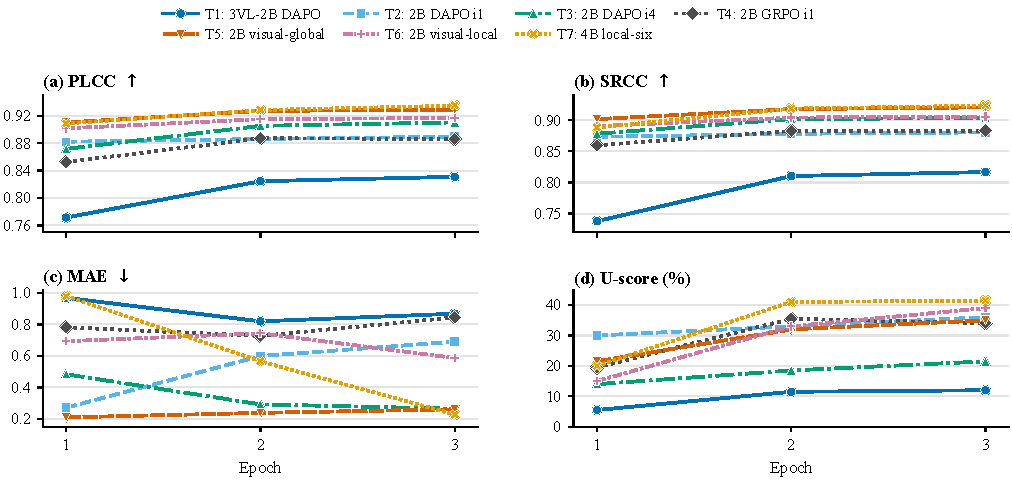
\includegraphics[width=\textwidth]{Figures/fig_ablation_epochs}
\caption{Validation trajectories through E3 on the common 200-image set. T7
denotes the 4B local-six run. Curves are single fixed-seed runs, so no error
bands are shown. Higher PLCC/SRCC and
lower MAE are better, while U-score diagnoses rating diversity. Color, marker,
and line style consistently identify T1--T7.}
\label{fig:ablation-epochs}
\end{figure*}

\begin{figure*}[!t]
\centering
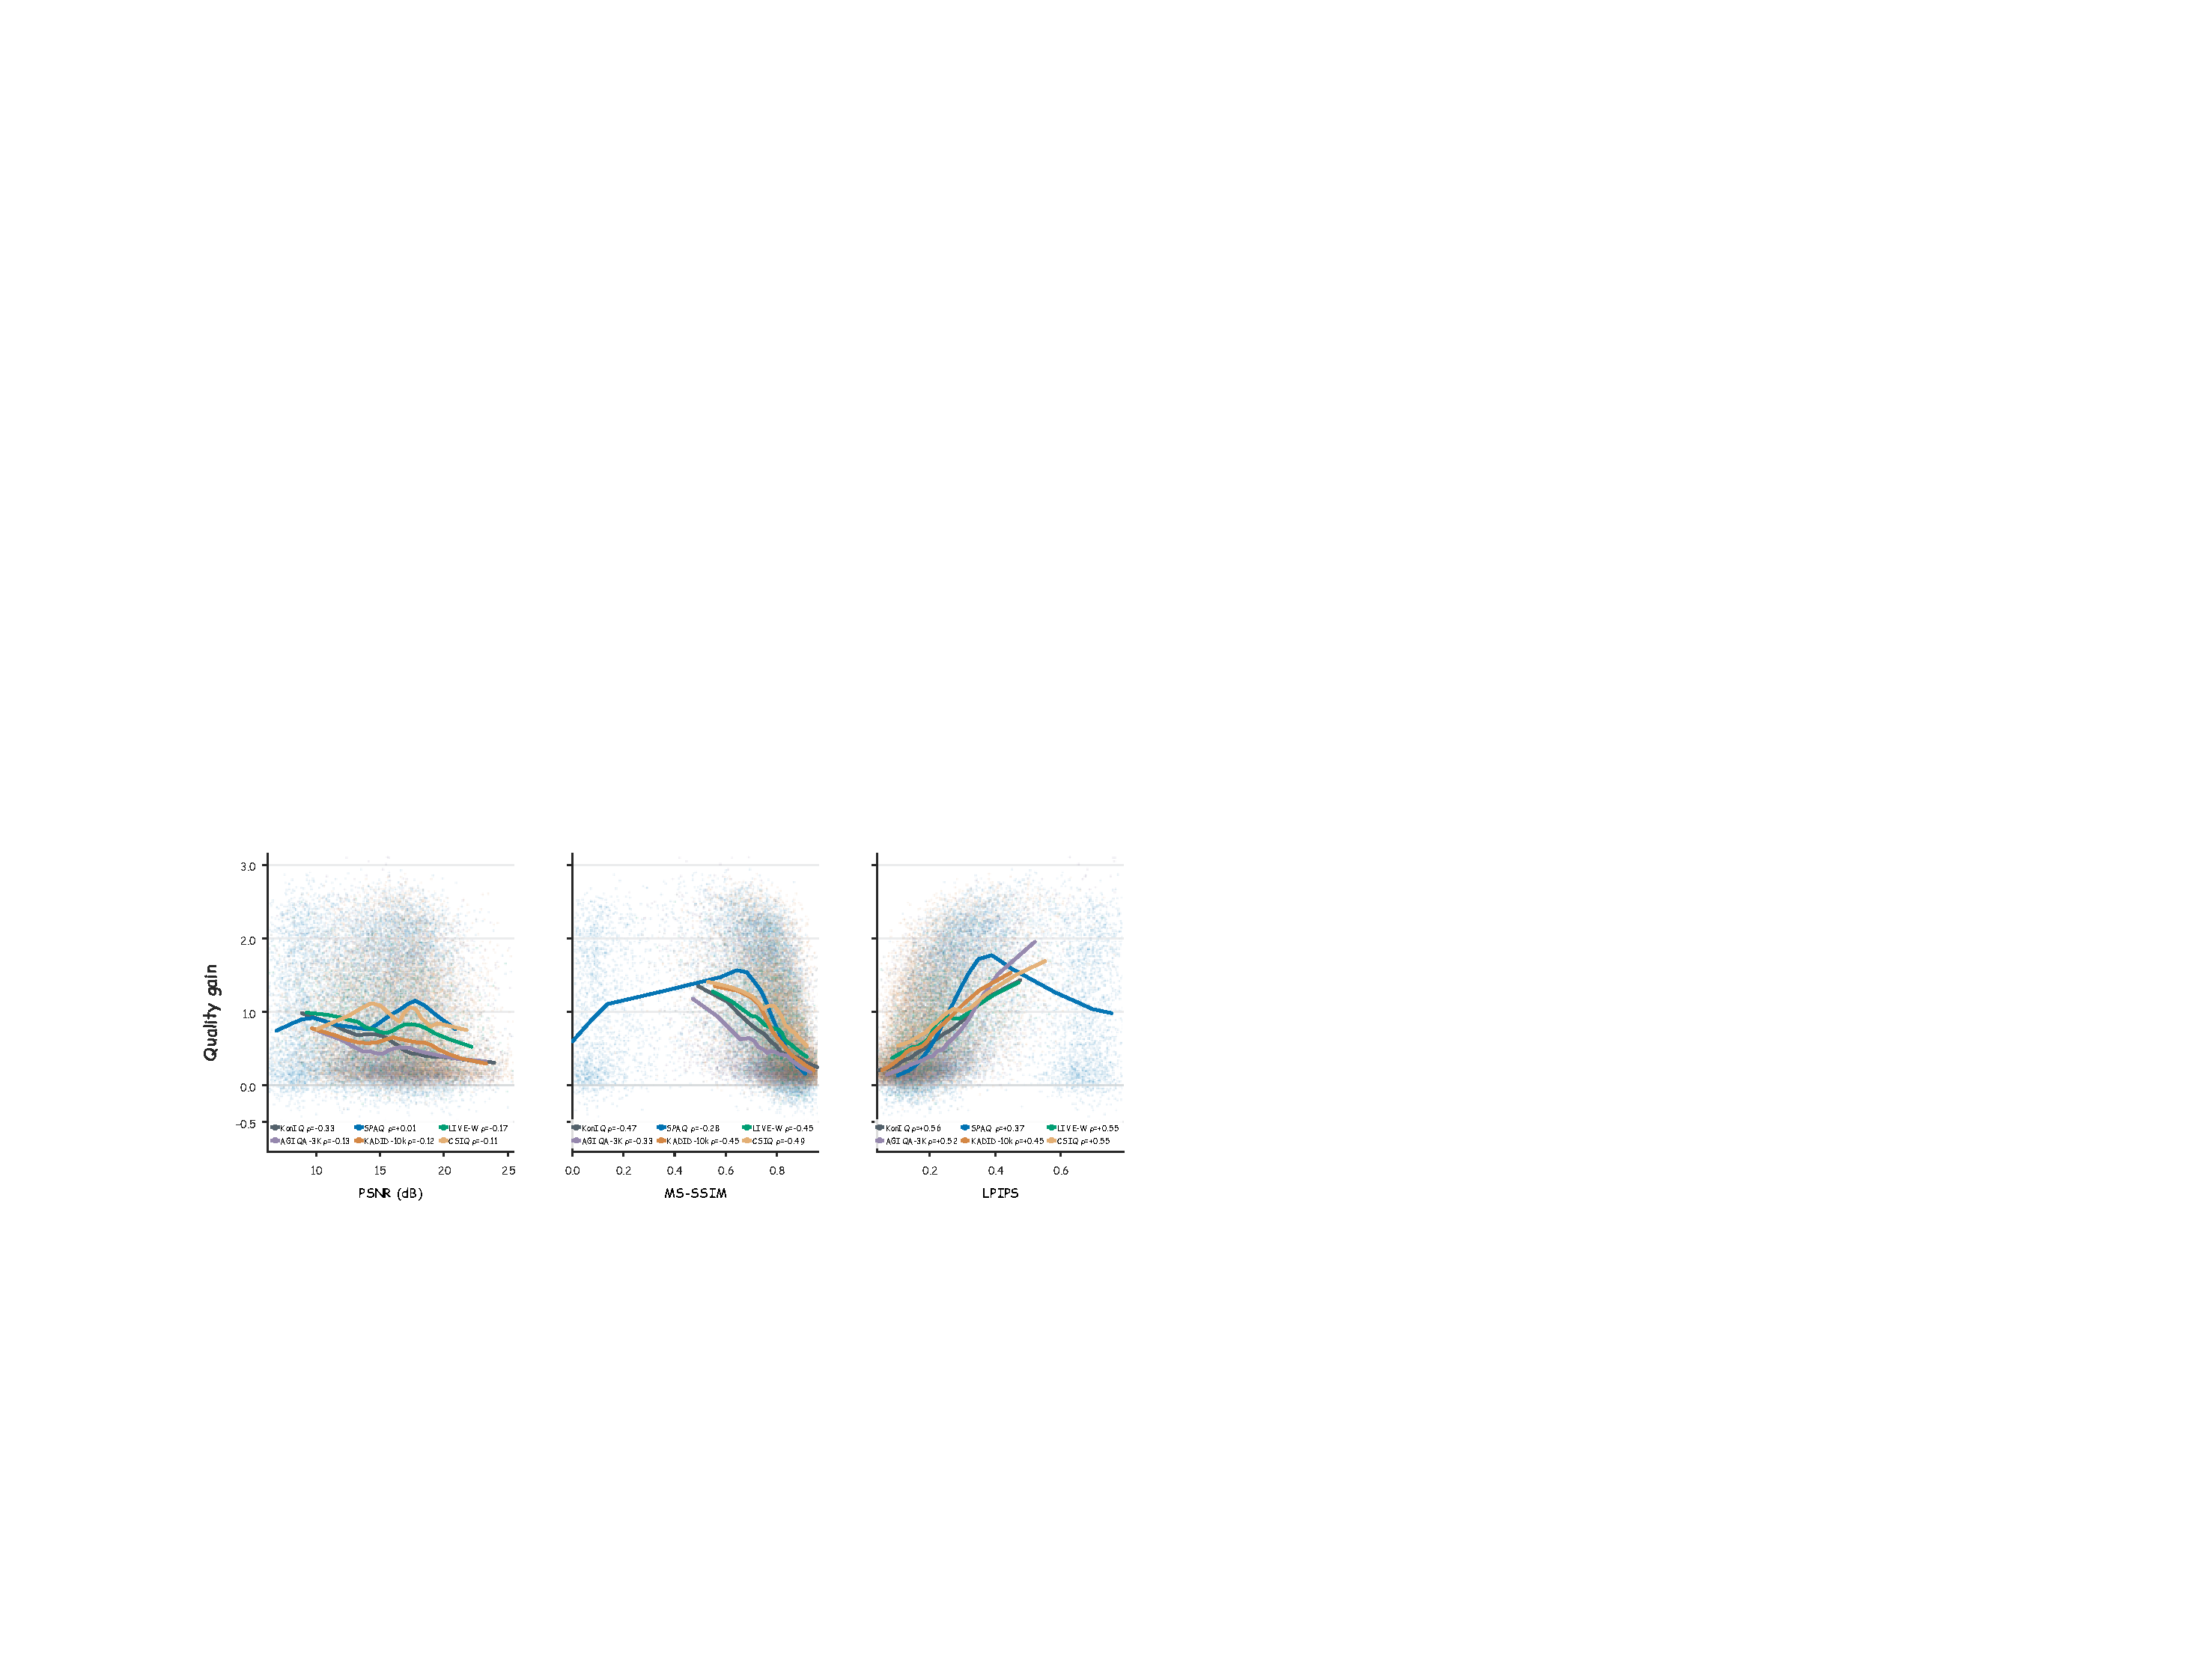
\includegraphics[width=\textwidth]{Figures/af2_analysis}
\caption{\textbf{Quality gain versus visual change scale.}
The panels relate the Judge-observed quality gain $\Delta s$ to PSNR,
MS-SSIM~\citep{wang2003msssim}, and LPIPS~\citep{zhang2018lpips} between the
original and edited images. Colors denote datasets, curves show smoothed
trends, and $\rho$ denotes Spearman correlation.}
\label{fig:quality-fidelity}
\end{figure*}

\subsection{Optimization Algorithms: GRPO or DAPO?}
\label{app:optimization-algorithms}

Compared with GRPO~\citep{shao2024deepseekmath},
DAPO~\citep{yu2025dapo} dynamically resamples low-variance groups, thereby
increasing within-group reward diversity and preventing policy advantages from
vanishing prematurely. We therefore adopted DAPO in most of our early
experiments.

Across three epochs, 3,282 of 20,832 GRPO learner groups (15.75\%) have zero
within-group reward variance and therefore zero policy advantage. DAPO
resampling reduces the proportion of zero-advantage learner groups to 0\%.
Comparing T2 and T4 in Table~\ref{tab:preliminary-ablation}, DAPO improves
the six-dataset macro PLCC/SRCC by 0.006/0.008 and reduces MAE by 0.138 at
Epoch 3, with improvements on five, six, and six datasets, respectively.

Despite its better performance, DAPO requires 1.866$\times$ more sampled
trajectories and increases the training time per epoch from 0.81 to 1.13 hours
(approximately 39.5\%). This additional training-time cost is
not affordable in our training environment, especially when scaling the model
to 4B parameters or beyond. Therefore, we use GRPO as the default optimization
algorithm in the final framework.

\subsection{Hyper-Parameter Settings.}

\paragraph{Group Size: 6 versus 48.}
MR-IQA~\citep{mr-iqa} reports its best performance with local groups of six,
where rewards are computed by comparing samples only within each six-image
group. Table~\ref{tab:preliminary-ablation} compares this local-6 setting (T6)
with a larger group of 48 (T5).
The large group achieves better in-domain validation PLCC/SRCC/MAE
(0.929/0.921/0.261 versus 0.917/0.906/0.587), whereas local-6 achieves higher
six-dataset macro PLCC/SRCC (0.835/0.813 versus 0.828/0.809). Because the
local-6 setting provides stronger cross-dataset correlation, we adopt a group
size of six.

\paragraph{Vision Modules: Frozen versus Active.}
The T2--T5 comparison in Table~\ref{tab:preliminary-ablation} shows that active
visual training performs better on authentic datasets, achieving
PLCC/SRCC values of 0.952/0.938 on KonIQ and 0.897/0.877 on LIVE-W, compared
with 0.925/0.904 and 0.881/0.847 for the frozen variant. In contrast, freezing
the vision encoder and aligner performs better on AGIQA-3K and the synthetic
datasets: it achieves 0.826/0.768 on AGIQA-3K, 0.665/0.676 on KADID-10k, and
0.840/0.801 on CSIQ, compared with 0.816/0.747, 0.661/0.668, and 0.771/0.746
under active visual training. Consequently, the frozen variant yields higher
six-dataset average PLCC/SRCC (0.840/0.816 versus 0.833/0.812), indicating
stronger overall generalization.

\paragraph{Rating Diversity.}
Zoom-IQA~\citep{zoom-iqa} reports score-space collapse when using a ranking
reward, with only a 2.04\% unique-score ratio. Across T1--T7 in
Table~\ref{tab:preliminary-ablation}, the E3 U-scores remain between 12.0\% and
41.5\%, corresponding to 24--83 distinct ratings on the 200-image validation
set. Thus, we do not observe rating-diversity collapse under our current
settings.

\paragraph{Repeated Sampling Updates.}
MR-IQA~\citep{mr-iqa} reuses each rollout sample for four policy updates. We
evaluate whether these repeated updates remain effective by comparing T2 and
T3 in Table~\ref{tab:preliminary-ablation}. Four updates improve validation
PLCC/SRCC/MAE from 0.890/0.881/0.691 to
0.910/0.904/0.265. However, the six-dataset macro PLCC/SRCC remain nearly
unchanged (0.835/0.808 versus 0.834/0.809), while training time increases from
1.13 to 2.47 hours per epoch. Therefore, one policy update per rollout is
sufficient under our current settings.

\section{Visual Quality Feature Analysis}
\label{app:visual-quality-feature-analysis}

In our framework, the FLUX.2 [klein] Editor~\citep{flux2} produces an edited
image conditioned on the quality reasoning for each input. The resulting
original--edited pair bridges single-image quality assessment with
reference-based quality assessment, enabling us to analyze how the visual
intervention relates to the predicted quality improvement. In this section, we
investigate three questions: (1) whether larger visual changes lead to greater
quality gains; (2) how the distributions of low-level visual features change
after editing; and (3) what behavioral preferences emerge from the overall
framework.

\subsection{Visual Change and Quality Gains}
\label{app:quality-fidelity}

\paragraph{Visual change and quality improvement.}
Figure~\ref{fig:quality-fidelity} relates the Judge-observed quality gain to
three reference-based measures of the visual change between the original and
edited images. Quality gain is generally negatively correlated with PSNR
($\rho=-0.33$ to $+0.01$) and MS-SSIM ($\rho=-0.49$ to $-0.28$), and
positively correlated with LPIPS ($\rho=0.37$ to $0.56$). Because larger
changes correspond to lower
PSNR/MS-SSIM and higher LPIPS, these consistent directions indicate that
larger editing changes are generally associated with greater image-quality
improvements. SPAQ deviates from the other datasets across multiple measures. Its
quality-gain correlation is nearly zero for PSNR ($\rho=+0.01$) and is the
weakest in magnitude for both MS-SSIM ($\rho=-0.28$) and LPIPS
($\rho=+0.37$). A similar pattern appears in rating performance: while the
rating correlations on the other datasets change during training, the SPAQ
correlation remains close to 0.90 with only minor variation. This stability
suggests that SPAQ is less sensitive to the training-induced changes observed
on the other benchmarks.

\subsection{Low-Level Visual Feature Patterns}
\label{app:quality-low-level-features}

\begin{figure*}[t!]
\centering
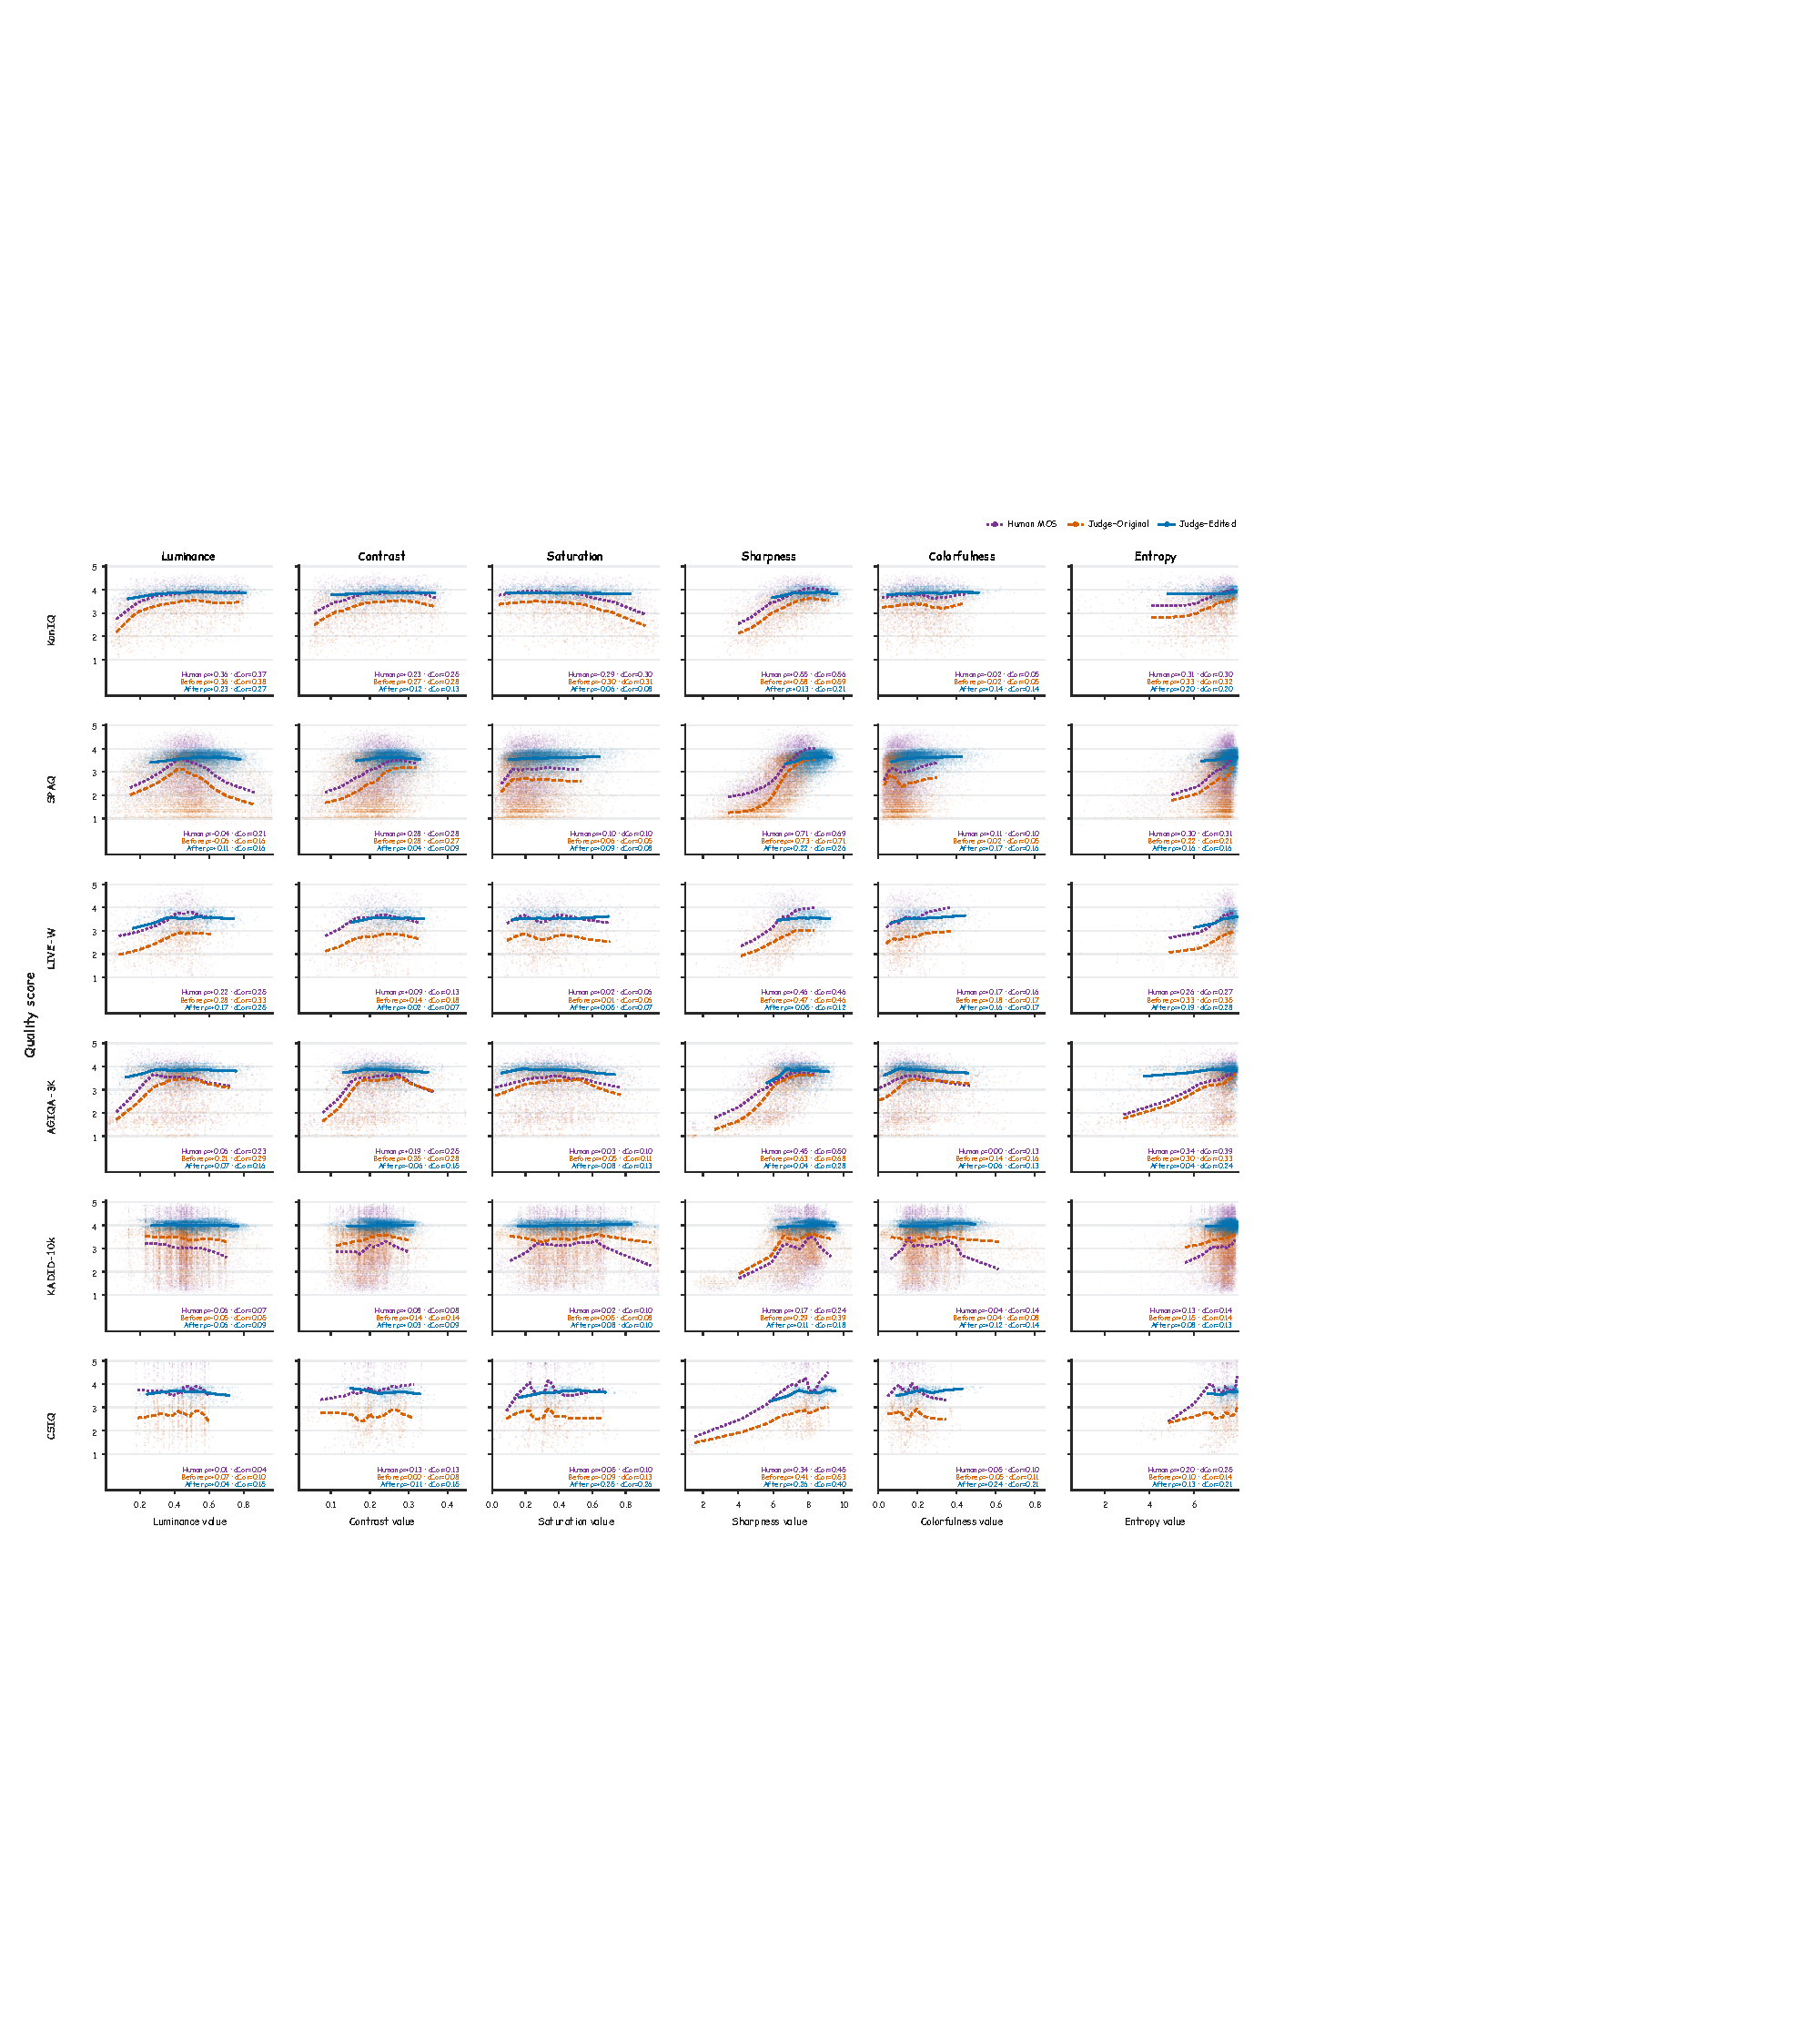
\includegraphics[width=\textwidth]{Figures/af1_figures_analysis.pdf}
\caption{\textbf{Quality scores versus low-level image features.} Rows denote
datasets and columns denote luminance, contrast, saturation, sharpness,
colorfulness, and entropy. Purple and orange show human MOS and Judge scores
for original images, while blue shows Judge scores for edited images. Curves
show smoothed trends; $\rho$ and dCor denote Spearman and distance
correlations~\citep{szekely2007distance}.}
\label{fig:quality-low-level-features}
\end{figure*}

\paragraph{Human-like Judge feedback.}
Figure~\ref{fig:quality-low-level-features} shows that the feature-dependent
curves produced by the original-image Judge broadly follow the corresponding
human-MOS curves across the six datasets. Their similar shapes and directions,
particularly for sharpness and contrast, indicate that the Judge captures
human-like quality preferences over low-level visual attributes. This
agreement supports its use as a qualified source of human-like feedback for
the original--edited image pairs.

\paragraph{Cross-dataset feature patterns.}
Among luminance, contrast, saturation, sharpness, colorfulness, and entropy,
sharpness exhibits the clearest cross-dataset trend. Both human MOS and Judge
scores generally increase with sharpness, whereas the other attributes show
weaker, nonlinear, or dataset-dependent patterns. This result suggests that
sharpness is a broadly shared quality cue, while no single low-level attribute
fully explains perceptual quality across all datasets.

\paragraph{Edited-feature distributions.}
After editing, the images retain broad distributions across all six low-level
attributes rather than collapsing to fixed feature values. The framework
therefore does not appear to overfit a single low-level pattern when improving
image quality. Nevertheless, Figure~\ref{fig:quality-low-level-features}
examines each attribute marginally. The joint distribution of low-level
attributes, and its relation to the human visual system and learned perceptual
representations such as CLIP-IQA~\citep{wang2023exploring}, warrants further
investigation.

\subsection{Framework Behavior Preference}

\begin{figure*}[p]
\centering
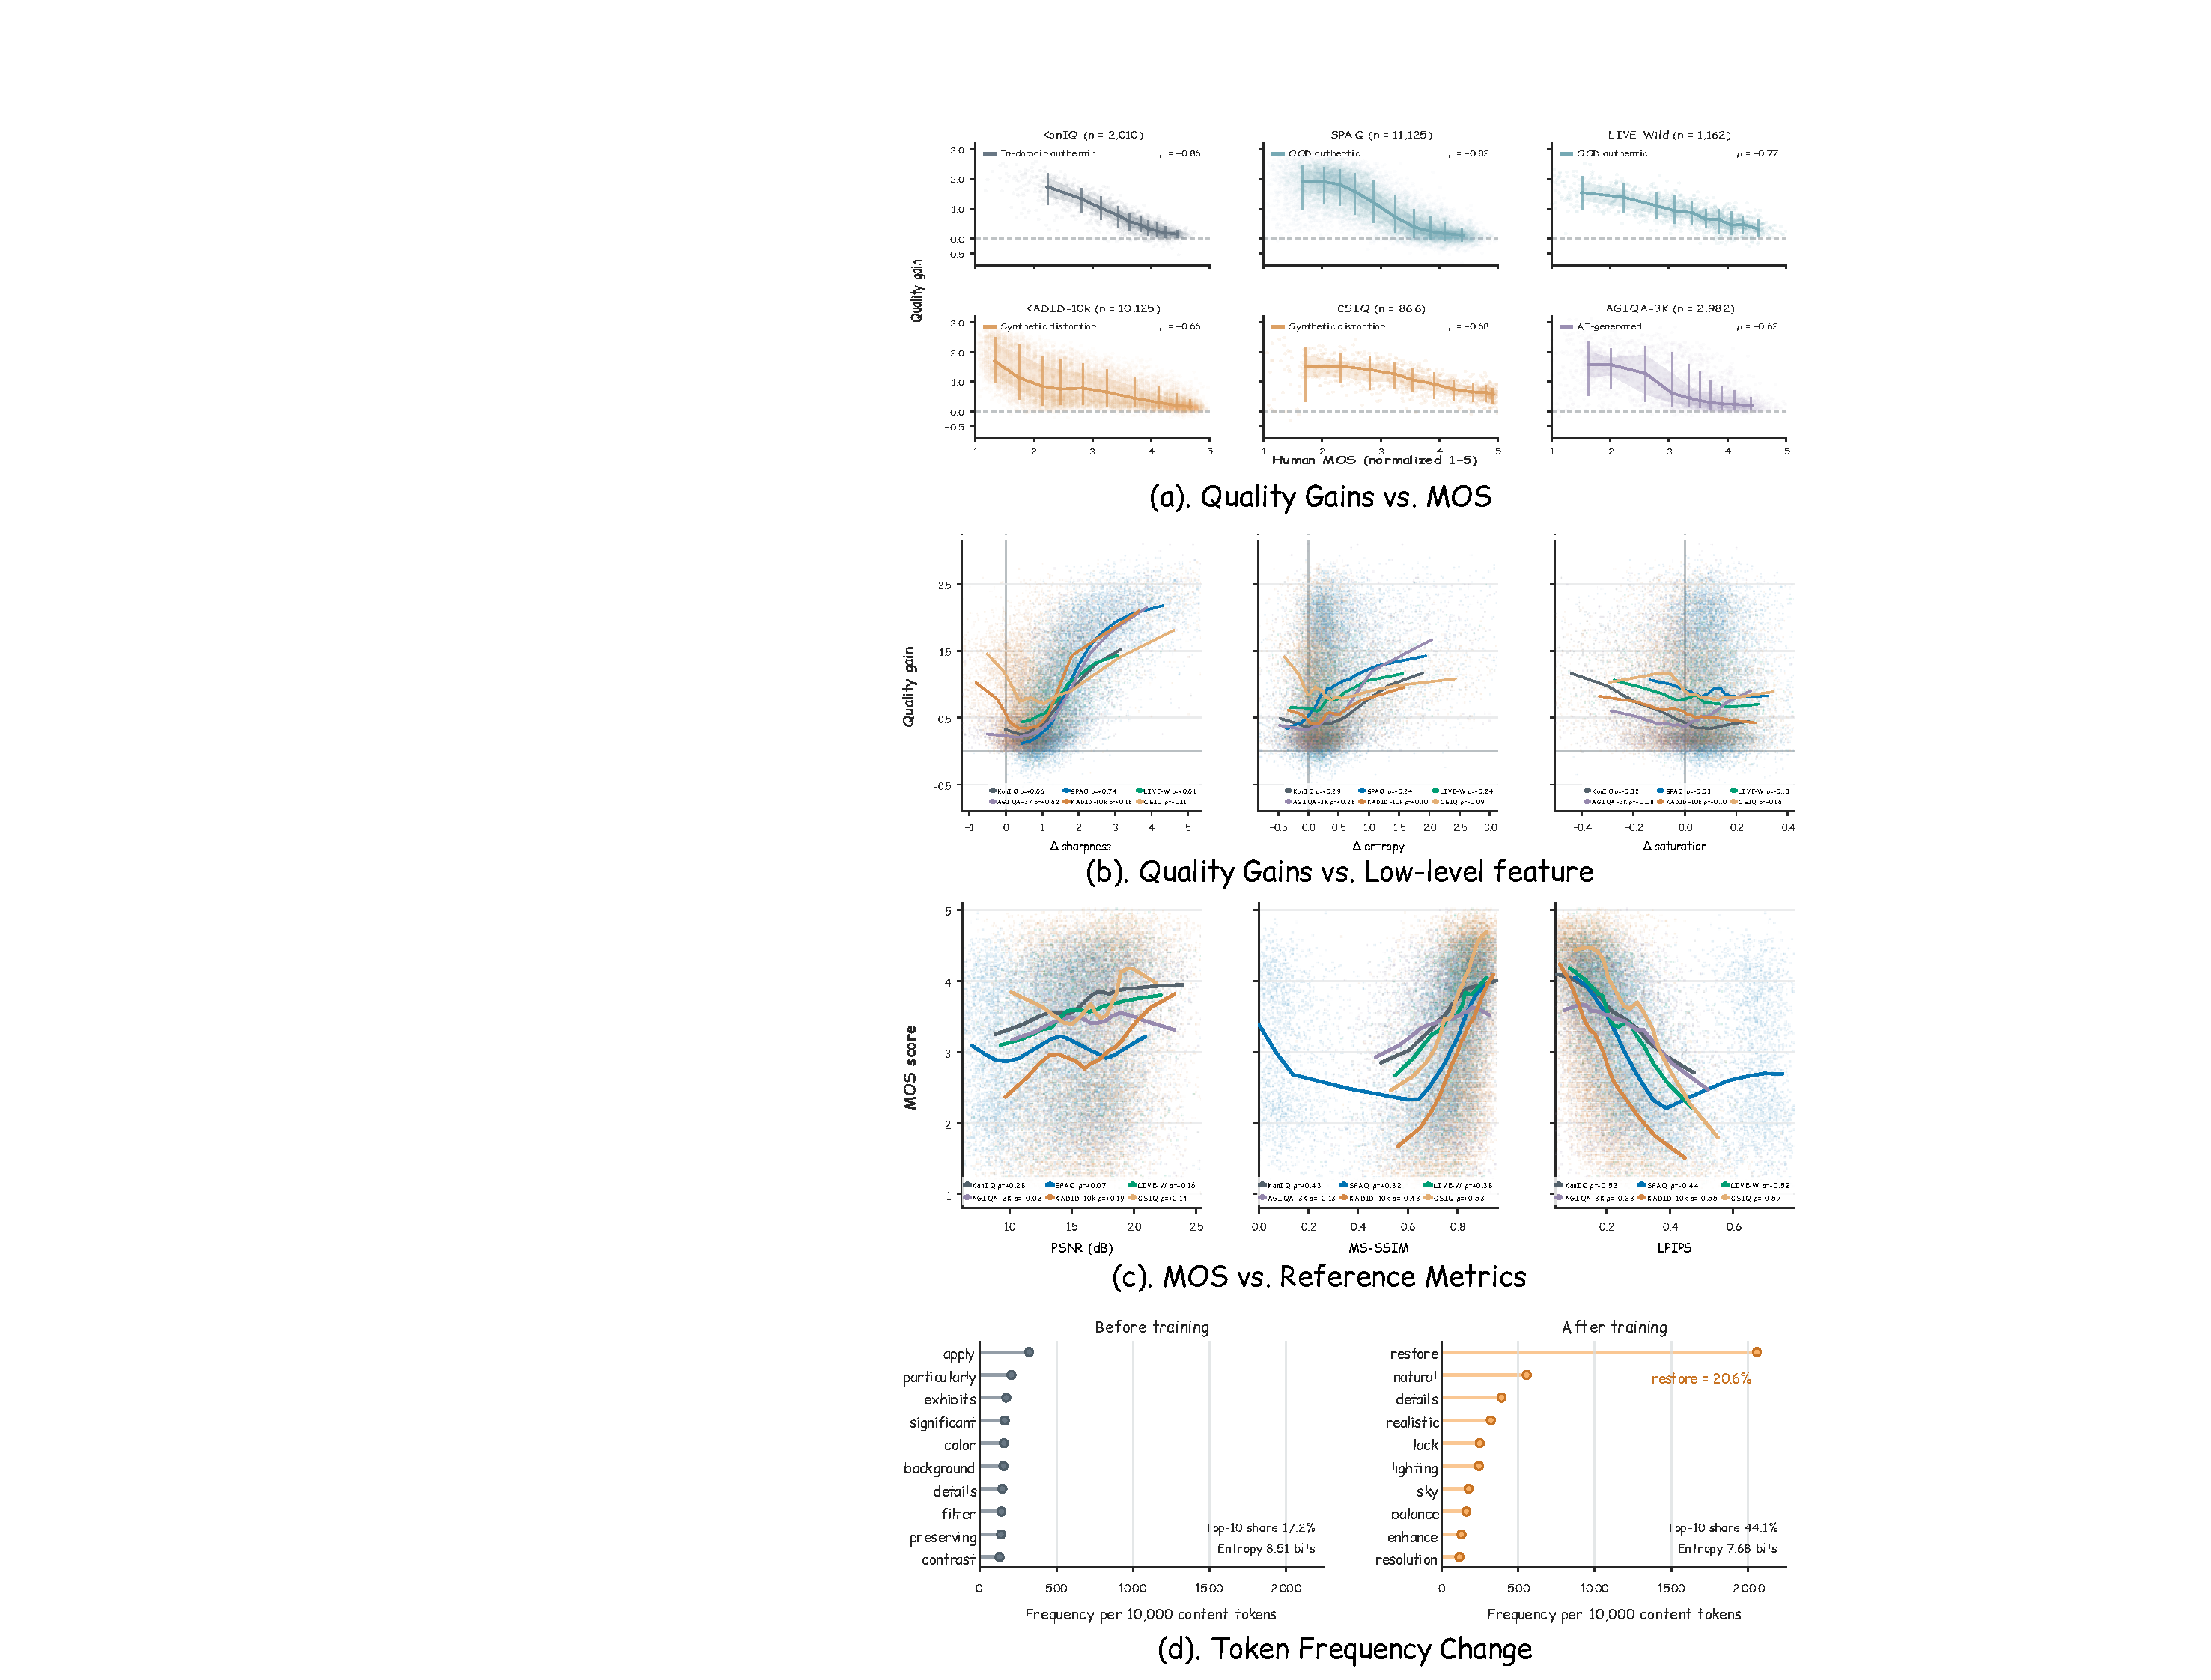
\includegraphics[
    height=0.90\textheight,
    keepaspectratio,
    pagebox=cropbox
]{Figures/af_4_figures_analysis.pdf}
\caption{\textbf{Behavioral analysis of reasoning-guided editing.}
(a) Judge-rated quality gain versus human MOS across six benchmarks.
(b) Quality gain versus changes in low-level image features.
(c) Human MOS versus reference-based similarity metrics between the original
and edited images.
(d) Frequent reasoning tokens before and after training.}
\label{fig:feature-analysis}
\end{figure*}

\paragraph{Source quality, visual change, and quality gain.}
Figure~\ref{fig:feature-analysis}(a) shows that lower-MOS images generally
receive larger Judge-rated quality gains. Panel (c) further shows that
lower-MOS images tend to have lower similarity between the original and edited
images, indicating larger visual changes. Together with the observation in
Section~\ref{app:quality-fidelity} that larger visual changes are associated
with higher quality gains, these results suggest a plausible behavior:
for lower-quality inputs, the model tends to modify more visual attributes,
which in turn leads to greater quality improvements. This behavior aligns with
the intuition that lower-quality images provide more room for correction and
supports the intended operation of our framework, although the observed
associations do not by themselves establish causality.

\paragraph{Preferences over feature changes.}
Unlike Section~\ref{app:quality-low-level-features}, which examines the
absolute values of low-level attributes, Figure~\ref{fig:feature-analysis}(b)
relates their changes after editing to the resulting quality gain. Changes in
sharpness retain the strongest and most consistent relationship with quality
improvement. For entropy and saturation, the authentic and synthetic datasets
form different response patterns, indicating that the preferred corrections
depend on the degradation domain. SPAQ again exhibits signals that are less
consistent with the other datasets, in agreement with the dataset-specific
behavior observed in Section~\ref{app:quality-fidelity}.

\paragraph{Behavioral adaptation and concentration.}
Figure~\ref{fig:feature-analysis}(d) reflects how the model adjusts its
reasoning vocabulary in response to Judge feedback. After training, terms such
as \emph{natural} and \emph{realistic} become prominent, revealing a learned
preference for perceptually plausible corrections. At the same time,
\emph{restore} alone accounts for 20.6\% of the displayed token frequency, and
the top-10 token share rises to 44.1\%. This concentration suggests an emerging
tendency to overfit a small set of solution patterns, despite the broader
behavioral alignment induced by the framework.

\section{Discussion on the Editor Proxy}
\label{app:editor-proxy}

This work does not disentangle the Editor's instruction-following capability
from semantic preservation, creating two attribution risks. First, quality may
degrade because of Editor limitations rather than an incorrect Actor
instruction. Second, the edited image may become semantically inconsistent
with the input, weakening quality change as a proxy for reasoning faithfulness.
Future work should use independent human or human-like evaluation to assess
instruction following, semantic consistency, and perceptual quality
separately, yielding more reliable feedback and a more faithful framework.

\iffalse
% Temporarily omitted from the supplementary material.
\begin{table*}[t]
\centering
{\small
\setlength{\tabcolsep}{3pt}
\renewcommand{\arraystretch}{0.96}
\begin{tabular}{@{}p{0.13\textwidth}p{0.24\textwidth}p{0.25\textwidth}p{0.33\textwidth}@{}}
\toprule
\textbf{Failure} & \textbf{Diagnostic evidence} & \textbf{Root cause} &
\textbf{Corrective measure} \\
\midrule
{\raggedright Edit-action collapse\par} &
Rating accuracy remained high, but every action was \texttt{no\_edit};
homogeneous six-sample groups had zero advantage. &
Within-group normalization cannot correct a homogeneous action and therefore
starves downstream edit-gain credit. &
Add counterfactual negative credit and low-quality resampling. Because edit
behavior did not recover, disable editing in the controlled actor-only
experiments. \\
\addlinespace[1pt]
{\raggedright Rating drift and invalid output\par} &
Ratings collapsed to 5.283 or shifted to 8--9.45 while pairwise ordering
remained informative. &
Reward parsing and validation used inconsistent validity rules. A pairwise
objective is also invariant to a global rating shift. &
Use one strict rating-range contract without reward-side clamping. Reject
invalid outputs and apply an absolute anchor only to homogeneous error groups. \\
\addlinespace[1pt]
{\raggedright Token-credit drift\par} &
Decoding and re-encoding generated IDs changed tokenization and shifted the
supervised field span. &
\texttt{encode(decode(ids))} is not guaranteed to reproduce the sampled token
sequence. &
Project field spans onto the original generated-token boundaries and use
prefix decoding only as a fallback for byte-split Unicode tokens. \\
\addlinespace[1pt]
{\raggedright Reward-variance collapse\par} &
1,513 of 1,536 groups had zero reward variance; only 138 of 9,216 completions
carried usable group advantage. &
Late-stage outputs became homogeneous. Additional sampling rounds did not
recover enough informative groups. &
Cap resampling, retain every complete effective group, and use complete
no-advantage groups only as zero-weight shape padding. Report effective-group
statistics explicitly. \\
\addlinespace[1pt]
{\raggedright Distributed underfill\par} &
With 282 effective rows, only one rank inserted padding and the distributed
token counts disagreed (7,046 versus 7,210). &
A rank-local predicate controlled a globally shared shape and normalization
path. &
All-reduce padding counts before branching, then execute the same physical-batch
and effective-token normalization path on every rank. \\
\addlinespace[1pt]
{\raggedright Schema and evaluation drift\par} &
Valid two-field outputs were parsed with an obsolete three-field schema; an old
SPAQ evaluation parsed only 34.07\% of ratings. &
Monitoring and evaluation did not share the schema, prompt, message template,
and backend used during training. &
Read schema from recorded trajectories and configuration, align the inference
contract with training, and report coverage together with PLCC, SRCC, and MAE. \\
\bottomrule
\end{tabular}
}
\caption{Method-relevant training failures and corrective measures. Values are
observed diagnostics, not benchmark results.}
\label{tab:training-failures}
\end{table*}

\FloatBarrier
\section{Technical Reports of Training Failures}
\label{app:training-failures}

\paragraph{Residual Limitation.}
The no-edit state remains unresolved: counterfactual credit was directionally
correct in 403 of 408 low-quality cases, but editing did not recover. Actor-only
ablations therefore omit editing and do not validate the full framework.
\fi

\FloatBarrier
\begin{figure*}[!t]
\centering
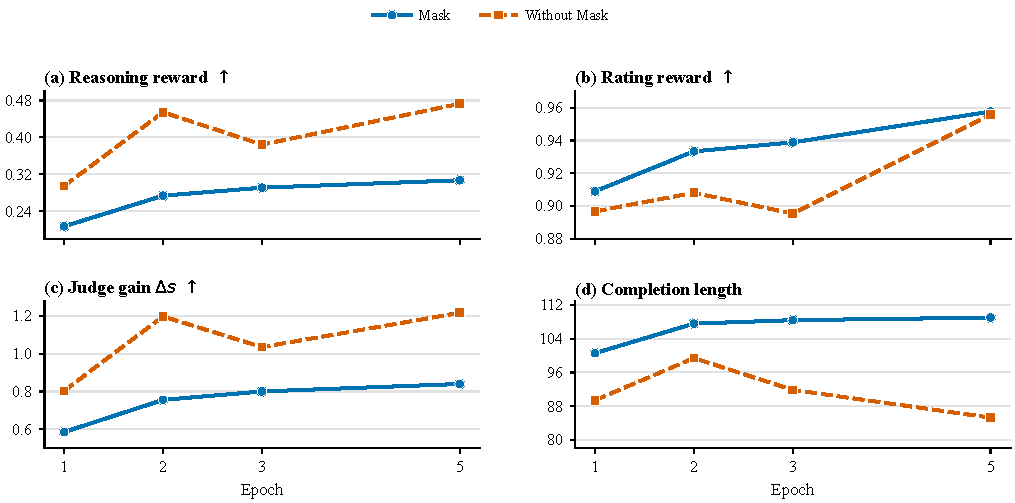
\includegraphics[width=0.85\textwidth]{Figures/fig_completion_audit_training.pdf}
\caption{\textbf{Training dynamics at the retained checkpoints.} Each point is
the exact four-rank mean for E1, E2, E3, or E5. Without Mask produces larger
reasoning reward and Judge gain, whereas rating reward converges similarly.
Its concurrent reduction in completion length is consistent with convergence
toward a high-reward solution template.}
\label{fig:credit-mask-training}
\end{figure*}

\section{Detailed Credit-Mask Audit}
\label{app:credit-mask-audit}

\subsection{Audit Scope and Protocol}
We audit two complete five-epoch runs with the same Actor, data, prompt, and
GRPO settings. \textbf{Mask} routes each reward to its supervised output with
output-specific KL regularization; \textbf{Without Mask} broadcasts rewards
over the complete output with one global KL term. Both use a KL coefficient of
$0.02$. The diagnostic reasoning reward bounds the raw Judge-score change:
\begin{equation}
    R_{i,k}^{\mathrm{diag}}
    =\operatorname{sgn}(\Delta s_{i,k})
    \left(1-\mathrm{e}^{-\Delta s_{i,k}^{2}/2}\right).
    \label{eq:diagnostic-reasoning-reward}
\end{equation}
The Editor consumes only the solution without an explicit semantic guardrail.
Both runs use six samples per image, 160-token completions, and frozen vision
encoder and aligner. Each contains 1,455 steps with 144 trajectories per step
(209,520 per run; 419,040 total). No step or record is missing, duplicated,
invalid, or non-finite. At Without Mask steps 711 and 713, all samples are
Actor-ineligible, so absent Judge changes reflect eligibility rather than
numerical or service failure. Because credit and KL routing change jointly and
each setting has one seed, this audit is descriptive rather than causal.

\subsection{Training Dynamics}
Figure~\ref{fig:credit-mask-training} reports exact four-rank means at the
retained checkpoints. Both configurations improve rating reward. Without Mask
produces larger reasoning reward and Judge gain, but also shorter outputs and
solution collapse. Mask changes more gradually: its reasoning reward rises
from 0.207 to 0.307 and Judge gain from 0.586 to 0.840. Rating rewards converge
by E5. KL losses are not directly comparable because their token scopes differ.
For Without Mask, mean reasoning reward and Judge gain increase from 0.463 and
1.189 over steps 1256--1355 to 0.478 and 1.232 over steps 1356--1455. Yet their
final-window slopes are $-0.0108$ and $-0.0246$; the rating-reward slope is
$-0.0006$. The endpoint therefore masks a plateau and slight decline.

\subsection{Checkpoint Validation}
Figure~\ref{fig:credit-mask-validation} evaluates the retained checkpoints on
the same 200 images. PLCC and SRCC improve for both runs. Without Mask keeps a
Judge gain near 1.18, while normalized-solution uniqueness falls from 91.88\%
at E1 to about 0.5\% at E2. The audit further shows that the semantic
dwelling-template rate reaches 100\% at E1. Semantic collapse therefore
precedes near-exact lexical collapse.

\begin{figure*}[!t]
\centering
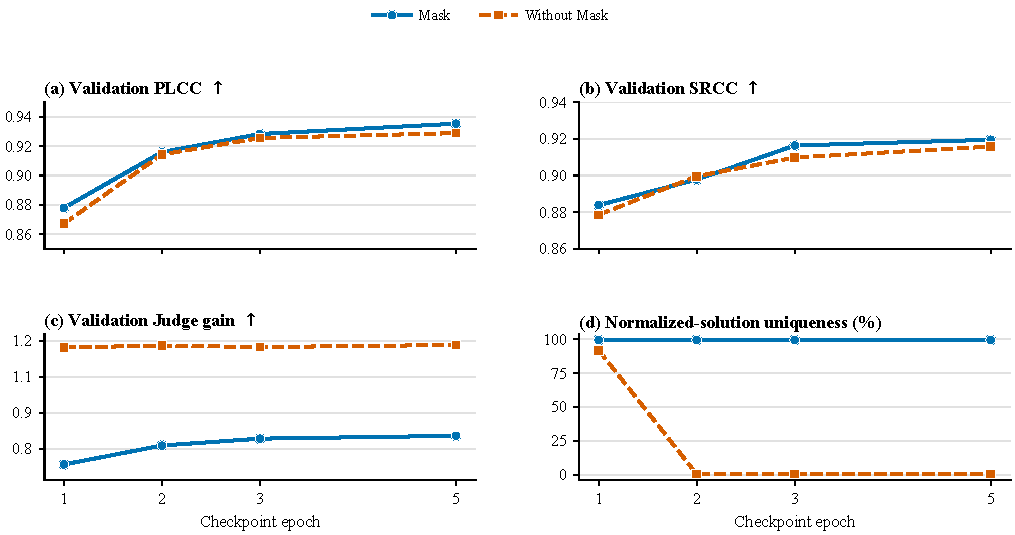
\includegraphics[width=0.85\textwidth]{Figures/fig_completion_audit_validation.pdf}
\caption{\textbf{Checkpoint validation dynamics.} Panels (a)--(c) report
PLCC, SRCC, and Judge gain on the complete 200-image validation set. Panel (d)
reports normalized-solution uniqueness. Without Mask maintains rating alignment
and high Judge gain while its solutions collapse.}
\label{fig:credit-mask-validation}
\end{figure*}

\subsection{Cross-Dataset Outcomes}
At E5, Without Mask obtains a larger pooled quality gain than Mask
($1.431$ versus $1.071$), although their six-dataset PLCC/SRCC averages remain
close ($0.834/0.812$ versus $0.838/0.812$). Larger gain alone therefore does not
establish healthier reasoning. All 28,270 Without Mask outputs share one
normalized solution; Mask retains 23,457 among 28,044 successful outputs.

\subsection{Collapse Milestones}
Table~\ref{tab:completion-audit-milestones} distinguishes semantic,
phrase-level, and near-exact collapse. Under Without Mask, the semantic
dwelling family exceeds 90\% at step 265, whereas one normalized sentence does
not exceed 90\% until step 551. Duplicate matching would detect the failure 286
steps late. Mask avoids dwelling collapse, although its super-resolution and
smoothing phrase backbone remains above 90\% from step 407 onward.

\begin{center}
\begin{minipage}{\columnwidth}
\centering
{\scriptsize
\setlength{\tabcolsep}{2.5pt}
\begin{tabular}{@{}p{1.55in}rrl@{}}
\toprule
\textbf{Routing and detector}
& $\boldsymbol{\geq 50\%}$ & $\boldsymbol{\geq 90\%}$
& \textbf{Sustained} \\
\midrule
Without Mask: semantic dwelling & 236 & 265 & 948--E5 \\
Without Mask: strict target phrase & 356 & 475 & -- \\
Without Mask: modal normalized solution & 520 & 551 & 973--E5 \\
Without Mask: canonical sentence & 1,133 & 1,146 & -- \\
Mask: super-resolution + smoothing & 214 & 260 & 407--E5 \\
\bottomrule
\end{tabular}
}
\captionof{table}{\textbf{Collapse milestones in global optimizer steps.} Semantic
detectors identify shared concepts before normalized near-duplicate matching
identifies one sentence.}
\label{tab:completion-audit-milestones}
\end{minipage}
\end{center}

\subsection{Output-Length Evolution}
Panel (d) of Figure~\ref{fig:credit-mask-training} shows that the mean training
completion decreases from 89.39 to 85.26 tokens under Without Mask but rises
from 100.57 to 109.00 under Mask. On validation outputs, the corresponding
solution lengths change from 32.56 to 18.00 and from 37.85 to 50.94. The former
contraction is consistent with convergence to one reusable instruction.

\subsection{Rating and Diversity Diagnostics}
Without Mask retains a KonIQ PLCC/SRCC of $0.932/0.914$ despite solution
collapse. Ratings still vary: 2,009 of 2,010 complete JSON outputs are unique,
although all 2,010 solutions are identical after normalization. Rating
correlation and full-output uniqueness therefore miss solution collapse.
Evaluation must inspect the supervised output alongside image--solution
relevance and semantic preservation.

\subsection{Representative Validation Outputs}
The Without Mask E5 Actor produces different evidence and ratings for the
three examples, but all solutions normalize to one dwelling instruction.
Sample 1 still receives 0.865 reward because the fixed intervention raises the
Judge score from 2.37 to 4.37. Thus, the reward measures edited-image quality
without establishing source-image faithfulness.

\begin{center}
\begin{minipage}{\columnwidth}
\centering
{\small
\setlength{\tabcolsep}{5pt}
\begin{tabular}{@{}lrrrrr@{}}
\toprule
\textbf{Sample} & \textbf{Rating} & $\boldsymbol{J_0}$
& $\boldsymbol{J_1}$ & $\boldsymbol{\Delta s}$ & $\boldsymbol{R}$ \\
\midrule
1 & 1.68 & 2.37 & 4.37 & 2.00 & 0.865 \\
2 & 3.32 & 3.84 & 4.32 & 0.48 & 0.109 \\
3 & 2.65 & 3.02 & 4.36 & 1.34 & 0.593 \\
\bottomrule
\end{tabular}
}
\captionof{table}{Representative Without Mask validation outputs. Different evidence
and ratings lead to the same normalized solution.}
\label{tab:completion-audit-examples}
\end{minipage}
\end{center}

\subsection{Causal Scope}
The comparison changes credit and KL routing jointly with one seed per setting.
It establishes a reproducible failure mode for Without Mask/global KL, but not
the responsible change. Causal attribution requires a $2{\times}2$ grid of
Mask versus Without Mask and component versus global KL, with multiple seeds.

\FloatBarrier


\end{document}

\section{Camera-Ready Guidelines}

Congratulations on having a paper selected for inclusion in an AAAI Press proceedings or technical report! This document details the requirements necessary to get your accepted paper published using PDF\LaTeX{}. If you are using Microsoft Word, instructions are provided in a different document. AAAI Press does not support any other formatting software.

The instructions herein are provided as a general guide for experienced \LaTeX{} users. If you do not know how to use \LaTeX{}, please obtain assistance locally. AAAI cannot provide you with support and the accompanying style files are \textbf{not} guaranteed to work. If the results you obtain are not in accordance with the specifications you received, you must correct your source file to achieve the correct result.

These instructions are generic. Consequently, they do not include specific dates, page charges, and so forth. Please consult your specific written conference instructions for details regarding your submission. Please review the entire document for specific instructions that might apply to your particular situation. All authors must comply with the following:

\begin{itemize}
\item You must use the 2027 AAAI Press \LaTeX{} style file and the aaai2027.bst bibliography style files, which are located in the 2027 AAAI Author Kit (aaai2027.sty, aaai2027.bst).
\item You must complete, sign, and return by the deadline the AAAI copyright form (unless directed by AAAI Press to use the AAAI Distribution License instead).
\item You must read and format your paper source and PDF according to the formatting instructions for authors.
\item You must submit your electronic files and abstract using our electronic submission form \textbf{on time.}
\item You must pay any required page or formatting charges to AAAI Press so that they are received by the deadline.
\item You must check your paper before submitting it, ensuring that it compiles without error, and complies with the guidelines found in the AAAI Author Kit.
\end{itemize}

\section{Copyright}
All papers submitted for publication by AAAI Press must be accompanied by a valid signed copyright form. They must also contain the AAAI copyright notice at the bottom of the first page of the paper. There are no exceptions to these requirements. If you fail to provide us with a signed copyright form or disable the copyright notice, we will be unable to publish your paper. There are \textbf{no exceptions} to this policy. You will find a PDF version of the AAAI copyright form in the AAAI AuthorKit. Please see the specific instructions for your conference for submission details.

\section{Formatting Requirements in Brief}
We need source and PDF files that can be used in a variety of ways and can be output on a variety of devices. The design and appearance of the paper is strictly governed by the aaai style file (aaai2027.sty).
\textbf{You must not make any changes to the aaai style file, nor use any commands, packages, style files, or macros within your own paper that alter that design, including, but not limited to spacing, floats, margins, fonts, font size, and appearance.} AAAI imposes requirements on your source and PDF files that must be followed. Most of these requirements are based on our efforts to standardize conference manuscript properties and layout. All papers submitted to AAAI for publication will be recompiled for standardization purposes. Consequently, every paper submission must comply with the following requirements:

\begin{itemize}
\item Your .tex file must compile in PDF\LaTeX{} --- (you may not include .ps or .eps figure files.)
\item All fonts must be embedded in the PDF file --- including your figures.
\item Modifications to the style file, whether directly or via commands in your document may not ever be made, most especially when made in an effort to avoid extra page charges or make your paper fit in a specific number of pages.
\item No type 3 fonts may be used (even in illustrations).
\item You may not alter the spacing above and below captions, figures, headings, and subheadings.
\item You may not alter the font sizes of text elements, footnotes, heading elements, captions, or title information (for references and mathematics, please see the limited exceptions provided herein).
\item You may not alter the line spacing of text.
\item Your title must follow Title Case capitalization rules (not sentence case).
\item \LaTeX{} documents must use the Times-like serif text font provided automatically by the aaai2027 style file. You may not use Computer Modern or Palatino for the text of your paper, and you must not load \texttt{times} or any other text-font package in your preamble---the style file manages the text font automatically.
\item Your source must not require use of fonts for non-Roman alphabets within the text itself. If your paper includes symbols in other languages (such as, but not limited to, Arabic, Chinese, Hebrew, Japanese, Thai, Russian and other Cyrillic languages), you must restrict their use to bit-mapped figures. Fonts that require non-English language support (CID and Identity-H) must be converted to outlines or removed from the document (even if they are in a graphics file embedded in the document).
\item Two-column format in AAAI style is required for all papers.
\item The paper size for final submission must be US letter without exception.
\item The source file must exactly match the PDF.
\item The document margins may not be exceeded (no content should overflow into the margins or gutter).
\item The number of pages and the file size must be as specified for your event.
\item No document may be password protected.
\item Neither the PDFs nor the source may contain any embedded links or bookmarks (no hyperref or navigator packages).
\item Your source and PDF must not have any page numbers, footers, or headers (no pagestyle commands).
\item Your PDF must conform to PDF version 1.5 or higher.
\item Your \LaTeX{} sources archive must not contain unnecessary files (figures, extra .tex files, etc.).
\item Your graphics must be sized appropriately outside of \LaTeX{} (do not use the ``clip" or ``trim'' command) .
\end{itemize}

If you do not follow these requirements, your paper will be returned to you to correct the deficiencies.

\section{What Files to Submit}
You must submit the following items to ensure that your paper is published:
\begin{itemize}
\item A fully-compliant PDF file.
\item Your \LaTeX{} source file submitted as a \textbf{single} .tex file (do not use the ``input" command to include sections of your paper --- every section must be in the single source file). (The only allowable exception is .bib file, which should be included separately).
\item The bibliography (.bib) file(s).
\item Your source must compile on our system, which includes only standard \LaTeX{} 2020 TeXLive support files.
\item Only the graphics files used in compiling paper.
\item The \LaTeX{}-generated files (e.g. .aux,  .bbl file, PDF, etc.).
\end{itemize}

Your \LaTeX{} source will be reviewed and recompiled on our system (if it does not compile, your paper will be returned to you). \textbf{Do not submit your source in multiple text files.} Your single \LaTeX{} source file must include all your text, your bibliography (formatted using aaai2027.bst), and any custom macros.

Your files should work without any supporting files (other than the program itself) on any computer with a standard \LaTeX{} distribution.

\textbf{Do not send files that are not actually used in the paper.} Avoid including any files not needed for compiling your paper, including, for example, this instructions file, unused graphics files, style files, additional material sent for the purpose of the paper review, intermediate build files and so forth.

\textbf{Obsolete style files.} The commands for some common packages (such as some used for algorithms), may have changed. Please be certain that you are not compiling your paper using old or obsolete style files.

\textbf{Final Archive.} Place your source files in a single archive which should be compressed using .zip. The final file size may not exceed 10 MB.
Name your source file with the last (family) name of the first author, even if that is not you.


\section{Using \LaTeX{} to Format Your Paper}

The latest version of the AAAI style file is available on AAAI's website. Download this file and place it in the \TeX\ search path. Placing it in the same directory as the paper should also work. You must download the latest version of the complete AAAI Author Kit so that you will have the latest instruction set and style file.

\subsection{Document Preamble}

In the \LaTeX{} source for your paper, you \textbf{must} place the following lines as shown in the example in this subsection. Add or subtract author and address lines as necessary, and uncomment the portions that apply to you. In most instances, this is all you need to do to format your paper correctly. The aaai2027 style file automatically loads all required text fonts (\texttt{newtxtext} for serif, \texttt{helvet} for sans-serif, \texttt{courier} for monospaced); do not add \textbackslash usepackage\{times\}, \textbackslash usepackage\{helvet\}, \textbackslash usepackage\{courier\}, or any other font package, as doing so will conflict with the style.

Leave the setcounter for section number depth commented out and set at 0 unless you want to add section numbers to your paper. If you do add section numbers, you must uncomment this line and change the number to 1 (for section numbers), or 2 (for section and subsection numbers). The style file will not work properly with numbering of subsubsections, so do not use a number higher than 2.

\subsubsection{The Following Must Appear in Your Preamble}
\begin{quote}
\begin{scriptsize}\begin{verbatim}
\documentclass[letterpaper]{article}
% DO NOT CHANGE THIS
\usepackage{aaai2027} % DO NOT CHANGE THIS
\usepackage[hyphens]{url} % DO NOT CHANGE THIS
\usepackage{graphicx} % DO NOT CHANGE THIS
\urlstyle{rm} % DO NOT CHANGE THIS
\def\UrlFont{\rm} % DO NOT CHANGE THIS
\usepackage{natbib}  % DO NOT CHANGE THIS
\usepackage{caption}  % DO NOT CHANGE THIS
\frenchspacing % DO NOT CHANGE THIS
%
% Keep the \pdfinfo as shown here. There's no need
% for you to add the /Title and /Author tags.
\pdfinfo{
/TemplateVersion (2027.1)
}
\end{verbatim}\end{scriptsize}
\end{quote}

\subsection{Preparing Your Paper}

After the preamble above, you should prepare your paper as follows:
\begin{quote}
\begin{scriptsize}\begin{verbatim}
\begin{document}
\maketitle
\begin{abstract}
%...
\end{abstract}\end{verbatim}\end{scriptsize}
\end{quote}

\noindent If you want to add links to the paper's code, dataset(s), and extended version or similar this is the place to add them, within a \emph{links} environment:
\begin{quote}%
\begin{scriptsize}\begin{verbatim}
\begin{links}
  \link{Code}{https://aaai.org/example/guidelines}
  \link{Datasets}{https://aaai.org/example/datasets}
  \link{Extended version}{https://aaai.org/example}
\end{links}\end{verbatim}\end{scriptsize}
\end{quote}
\noindent Make sure that you do not de-anonymize yourself with these links if you are preparing an anonymous submission.

\noindent You should then continue with the body of your paper. Your paper must conclude with the references, which should be inserted as follows:
\begin{quote}
\begin{scriptsize}\begin{verbatim}
% References and End of Paper
% These lines must be placed at the end of your paper
\bibliography{Bibliography-File}
\end{document}
\end{verbatim}\end{scriptsize}
\end{quote}

\subsection{Commands and Packages That May Not Be Used}
\begin{table*}[t]
\centering

\begin{tabular}{llll}
  \toprule
  \textbackslash abovecaption &
  \textbackslash abovedisplay &
  \textbackslash addevensidemargin &
  \textbackslash addsidemargin \\
  \textbackslash addtolength &
  \textbackslash baselinestretch &
  \textbackslash belowcaption &
  \textbackslash belowdisplay \\
  \textbackslash break &
  \textbackslash clearpage &
  \textbackslash clip &
  \textbackslash columnsep \\
  \textbackslash float &
  \textbackslash linespread &
  \textbackslash newpage &
  \textbackslash pagebreak \\
  \textbackslash setlength &
  \textbackslash textheight &
  \textbackslash tiny &
  \textbackslash topmargin \\
  \textbackslash trim &
  \textbackslash vskip\{- &
  \textbackslash vspace\{- \\
  \bottomrule
\end{tabular}
\caption{Commands that must not be used}
\label{table1}
\end{table*}

\begin{table}[t]
\centering
\begin{tabular}{llll}
  \toprule
    authblk & babel & balance & cjk \\
    epsf & epsfig & euler & float \\
    fullpage & geometry & graphics & hyperref \\
    layout & lmodern & navigator & pdfcomment \\
    pgfplots & psfig & pstricks & t1enc \\
    times & titlesec & tocbibind & ulem \\
  \bottomrule
\end{tabular}
\caption{LaTeX style packages that must not be used.}
\label{table2}
\end{table}

There are a number of packages, commands, scripts, and macros that are incompatible with aaai2027.sty. The common ones are listed in tables \ref{table1} and \ref{table2}. Generally, if a command, package, script, or macro alters float spacings, margins, fonts, sizing, linespacing, or the presentation of the references and citations, it is unacceptable. Note that negative vskip and vspace may not be used except in certain rare occurrences, and may never be used around tables, figures, captions, sections, subsections, subsubsections, or references.


\subsection{Page Breaks}
For your final camera ready copy, you must not use any page break commands. References must flow directly after the text without breaks. Note that some conferences require references to be on a separate page during the review process. AAAI Press, however, does not require this condition for the final paper.


\subsection{Paper Size, Margins, and Column Width}
Papers must be formatted to print in two-column format on 8.5 x 11 inch US letter-sized paper. The margins must be exactly as follows:
\begin{itemize}
\item Top margin: 1.25 inches (first page), .75 inches (others)
\item Left margin: .75 inches
\item Right margin: .75 inches
\item Bottom margin: 1.25 inches
\end{itemize}


The default paper size in most installations of \LaTeX{} is A4. However, because we require that your electronic paper be formatted in US letter size, the aaai2027.sty style file enforces US letter page size automatically. Please note that using any other package to alter page size (such as, but not limited to the Geometry package) will result in your final paper being returned to you for correction.


\subsubsection{Column Width and Margins.}
To ensure maximum readability, your paper must include two columns. Each column should be 3.3 inches wide (slightly more than 3.25 inches), with a .375 inch (.952 cm) gutter of white space between the two columns. The aaai2027.sty file will automatically create these columns for you.

\subsection{Overlength Papers}
If your paper is too long and you resort to formatting tricks to make it fit, it is quite likely that it will be returned to you. The best way to retain readability if the paper is overlength is to cut text, figures, or tables. There are a few acceptable ways to reduce paper size that don't affect readability. First, turn on \textbackslash frenchspacing, which will reduce the space after periods. Next, move all your figures and tables to the top of the page. Consider removing less important portions of a figure. If you use \textbackslash centering instead of \textbackslash begin\{center\} in your figure environment, you can also buy some space. For mathematical environments, you may reduce fontsize {\bf but not below 6.5 point}.


Commands that alter page layout are forbidden. These include \textbackslash columnsep,  \textbackslash float, \textbackslash topmargin, \textbackslash topskip, \textbackslash textheight, \textbackslash textwidth, \textbackslash oddsidemargin, and \textbackslash evensizemargin (this list is not exhaustive). If you alter page layout, you will be required to pay the page fee. Other commands that are questionable and may cause your paper to be rejected include \textbackslash parindent, and \textbackslash parskip. Commands that alter the space between sections are forbidden. The title sec package is not allowed. Regardless of the above, if your paper is obviously ``squeezed" it is not going to to be accepted. Options for reducing the length of a paper include reducing the size of your graphics, cutting text, or paying the extra page charge (if it is offered).


\subsection{Type Font and Size}
Your paper must be formatted using the Times-like serif text font provided automatically by the aaai2027 style file (\texttt{newtxtext}). We will not accept papers formatted using Computer Modern or Palatino or some other text typeface. Do not load \texttt{times}, \texttt{helvet}, \texttt{courier}, or any other font package in your preamble; the style file loads all three automatically. Sans-serif text, when used, is Helvetica (\texttt{helvet}); monospaced text is Courier (\texttt{courier}). Use Symbol, Lucida, or Computer Modern for \textit{mathematics only.}

Do not use type 3 fonts for any portion of your paper, including graphics. Type 3 bitmapped fonts are designed for fixed resolution printers. Most print at 300 dpi even if the printer resolution is 1200 dpi or higher. They also often cause high resolution imagesetter devices to crash. Consequently, AAAI will not accept electronic files containing obsolete type 3 fonts. Files containing those fonts (even in graphics) will be rejected. (Authors using blackboard symbols must avoid packages that use type 3 fonts.)

Fortunately, the aaai2027 style file --- which loads \texttt{newtxtext}, \texttt{helvet}, and \texttt{courier} --- embeds Type~1 outlines automatically under PDF\LaTeX{}. Computer Modern used for mathematics is also fine: current TeX Live and MiKTeX distributions include cm-super and Latin Modern Type~1 fonts by default, so no manual font installation is required.

If you are unsure whether your paper contains Type~3 fonts, open the PDF in a viewer such as Adobe Acrobat Reader and inspect the font list (File $>$ Properties $>$ Fonts). Each embedded font should be listed as ``Type~1,'' ``TrueType,'' or ``OpenType'' --- not ``Type~3.'' The same inspection applies to embedded figures: export them from your illustration tool as PDF or high-resolution PNG/JPEG rather than EPS or PostScript.

The default size for your type must be ten-point with twelve-point leading (line spacing). Start all pages (except the first) directly under the top margin. (See the next section for instructions on formatting the title page.) Indent ten points when beginning a new paragraph, unless the paragraph begins directly below a heading or subheading.

\subsubsection{Nonroman Fonts.}
If your paper includes symbols in other languages (such as, but not limited to, Arabic, Chinese, Hebrew, Japanese, Thai, Russian and other Cyrillic languages), you must restrict their use to bit-mapped figures.

\subsection{Title and Authors}
Your title must appear centered over both text columns in sixteen-point bold type (twenty-four point leading). The title must be written in Title Case according to the Chicago Manual of Style rules. The rules are a bit involved, but in general verbs (including short verbs like be, is, using, and go), nouns, adverbs, adjectives, and pronouns should be capitalized, (including both words in hyphenated terms), while articles, conjunctions, and prepositions are lower case unless they directly follow a colon or long dash. You can use the online tool \url{https://titlecaseconverter.com/} to double-check the proper capitalization (select the "Chicago" style and mark the "Show explanations" checkbox).

Author's names should appear below the title of the paper, centered in twelve-point type (with fifteen point leading), along with affiliation(s) and complete address(es) (including electronic mail address if available) in nine-point roman type (the twelve point leading). You should begin the two-column format when you come to the abstract.

\subsubsection{Formatting Author Information.}
Author information has to be set according to the following specification depending if you have one or more than one affiliation. You may not use a table nor may you employ the \texttt{authorblk.sty} package. For one or several authors from the same institution, please separate them with commas and write all affiliation directly below (one affiliation per line) using the macros \textbackslash author and \textbackslash affiliations:

\begin{quote}\begin{scriptsize}\begin{verbatim}
\author{
    Author 1, ..., Author n\\
}
\affiliations {
    Address line\\
    ... \\
    Address line\\
}
\end{verbatim}\end{scriptsize}\end{quote}


\noindent For authors from multiple institutions, use \textbackslash textsuperscript \{\textbackslash rm x\} to link authors to their affiliations. Ensure there are no spaces between the author name and the superscript. The comma should be placed after the superscript.

\begin{quote}\begin{scriptsize}\begin{verbatim}
\author{
    AuthorOne\equalcontrib\textsuperscript{\rm 1,\rm 2},
    AuthorTwo\equalcontrib\textsuperscript{\rm 2},
    AuthorThree\textsuperscript{\rm 3},\\
    AuthorFour\textsuperscript{\rm 4},\\
    AuthorFive\textsuperscript{\rm 5}
}
\affiliations {
    \textsuperscript{\rm 1}AffiliationOne,\\
    \textsuperscript{\rm 2}AffiliationTwo,\\
    \textsuperscript{\rm 3}AffiliationThree,\\
    \textsuperscript{\rm 4}AffiliationFour,\\
    \textsuperscript{\rm 5}AffiliationFive\\
    \{email, email\}@affiliation.com,
    email@affiliation.com,
    email@affiliation.com,
    email@affiliation.com
}
\end{verbatim}\end{scriptsize}\end{quote}

You can indicate that some authors contributed equally using the \textbackslash equalcontrib command. This will add a marker after the author names and a footnote on the first page.

Similarly, you can mark author(s) as corresponding author(s) with the \textbackslash corresponding command within the \textbackslash author environment.

Note that you may want to  break the author list for better visualization. You can achieve this using a simple line break (\textbackslash  \textbackslash).

\subsection{\LaTeX{} Copyright Notice}
If you use aaai2027.sty in camera-ready mode the copyright notice is inserted automatically and may not be disabled. In submission mode the copyright disclaimer is automatically suppressed.

\subsection{Credits}
Any credits to a sponsoring agency should appear in the acknowledgments section, unless the agency requires different placement. If it is necessary to include this information on the front page, use
\textbackslash thanks in either the \textbackslash author or \textbackslash title commands.
For example:
\begin{quote}
\begin{small}
\textbackslash title\{Very Important Results in AI\textbackslash thanks\{This work is
 supported by everybody.\}\}
\end{small}
\end{quote}
Multiple \textbackslash thanks commands can be given. Each will result in a separate footnote indication in the author or title with the corresponding text at the bottom of the first column of the document. Note that the \textbackslash thanks command is fragile. You will need to use \textbackslash protect.

Please do not include \textbackslash pubnote commands in your document.

\subsection{Abstract}
Follow the example commands in this document for creation of your abstract. The command \textbackslash begin\{abstract\} will automatically indent the text block. Please do not indent it further. {Do not include references in your abstract!}

\subsection{Page Numbers}

Do not print any page numbers on your paper. The use of \textbackslash pagestyle is forbidden.

\subsection{Text}
The main body of the paper must be formatted in black, ten-point Times Roman with twelve-point leading (line spacing). You may not reduce font size or the linespacing. Commands that alter font size or line spacing (including, but not limited to baselinestretch, baselineshift, linespread, and others) are expressly forbidden. In addition, you may not use color in the text.

\subsection{Citations}
Citations within the text should include the author's last name and year, for example (Newell 1980). Append lower-case letters to the year in cases of ambiguity. Multiple authors should be treated as follows: (Feigenbaum and Engelmore 1988) or (Ford, Hayes, and Glymour 1992). In the case of four or more authors, list only the first author, followed by et al. (Ford et al. 1997).

\subsection{Extracts}
Long quotations and extracts should be indented ten points from the left and right margins.

\begin{quote}
This is an example of an extract or quotation. Note the indent on both sides. Quotation marks are not necessary if you offset the text in a block like this, and properly identify and cite the quotation in the text.

\end{quote}

\subsection{Footnotes}
Use footnotes judiciously, taking into account that they interrupt the reading of the text. When required, they should be consecutively numbered throughout with superscript Arabic numbers. Footnotes should appear at the bottom of the page, separated from the text by a blank line space and a thin, half-point rule.

\subsection{Headings and Sections}
When necessary, headings should be used to separate major sections of your paper. Remember, you are writing a short paper, not a lengthy book! An overabundance of headings will tend to make your paper look more like an outline than a paper. The aaai2027.sty package will create headings for you. Do not alter their size nor their spacing above or below.

\subsubsection{Section Numbers.}
The use of section numbers in AAAI Press papers is optional. To use section numbers in \LaTeX{}, uncomment the setcounter line in your document preamble and change the 0 to a 1. Section numbers should not be used in short poster papers and/or extended abstracts.

\subsubsection{Section Headings.}
Sections must appear in the following order:
\begin{enumerate}
\item Main content sections
\item Content Appendices (optional).  These appendices are considered part of the main paper, count towards page limits and and are subject to the same formatting and review requirements.
\item Ethical Statement (optional, unnumbered)
\item Acknowledgments (optional, unnumbered)
\item References (unnumbered)
\item Supplementary Material / Technical Appendices (only if permitted by the conference). Policies regarding supplementary material vary across conferences: some require technical appendices to be submitted as separate documents, some permit them at submission time but do not publish them in the proceedings, and others do not allow them at all. Consult the conference website for the applicable instructions.
\end{enumerate}

\subsubsection{Content Appendices.}
Content appendices must appear after the main content. If your main sections are numbered, appendix sections must use letters instead of arabic numerals. In \LaTeX{} you can use the \texttt{\textbackslash appendix} command to achieve this effect and then use \texttt{\textbackslash section\{Heading\}} normally for your appendix sections.

\subsubsection{Ethical Statement.}
You can write a statement about the potential ethical impact of your work, including its broad societal implications, both positive and negative. If included, such statement must be written in an unnumbered section titled \emph{Ethical Statement}.

\subsubsection{Acknowledgments.}
The acknowledgments section, if included, appears right before the references and is headed ``Acknowledgments". It must not be numbered even if other sections are (use \texttt{\textbackslash section*\{Acknowledgments\}} in \LaTeX{}). This section includes acknowledgments of help from associates and colleagues, credits to sponsoring agencies, financial support, and permission to publish. Please acknowledge other contributors, grant support, and so forth, in this section. Do not put acknowledgments in a footnote on the first page. If your grant agency requires acknowledgment of the grant on page 1, limit the footnote to the required statement, and put the remaining acknowledgments at the back. Please try to limit acknowledgments to no more than three sentences.

\subsubsection{References.}
The references section should be labeled ``References" and must appear at the very end of the paper (don't end the paper with references, and then put a figure by itself on the last page). A sample list of references is given later on in these instructions. Please use a consistent format for references. Poorly prepared or sloppy references reflect badly on the quality of your paper and your research. Please prepare complete and accurate citations.

\subsection{Illustrations and Figures}

\begin{figure}[t]
\centering
\includegraphics[width=0.9\columnwidth]{Figures/figure1} % Reduce the figure size so that it is slightly narrower than the column. Don't use precise values for figure width.This setup will avoid overfull boxes.
\caption{Using the trim and clip commands produces fragile layers that can result in disasters (like this one from an actual paper) when the color space is corrected or the PDF combined with others for the final proceedings. Crop your figures properly in a graphics program -- not in LaTeX.}
\label{fig1}
\end{figure}

\begin{figure*}[t]
\centering
\includegraphics[width=0.8\textwidth]{Figures/figure2} % Reduce the figure size so that it is slightly narrower than the column.
\caption{Adjusting the bounding box instead of actually removing the unwanted data resulted multiple layers in this paper. It also needlessly increased the PDF size. In this case, the size of the unwanted layer doubled the paper's size, and produced the following surprising results in final production. Crop your figures properly in a graphics program. Don't just alter the bounding box.}
\label{fig2}
\end{figure*}

% Using the \centering command instead of \begin{center} ... \end{center} will save space
% Positioning your figure at the top of the page will save space and make the paper more readable
% Using 0.95\columnwidth in conjunction with the


Your paper must compile in PDF\LaTeX{}. Consequently, all your figures must be .jpg, .png, or .pdf. You may not use the .gif (the resolution is too low), .ps, or .eps file format for your figures.

Figures, drawings, tables, and photographs should be placed throughout the paper on the page (or the subsequent page) where they are first discussed. Do not group them together at the end of the paper. If placed at the top of the paper, illustrations may run across both columns. Figures must not invade the top, bottom, or side margin areas. Figures must be inserted using the \textbackslash usepackage\{graphicx\}. Number figures sequentially, for example, figure 1, and so on. Do not use minipage to group figures.

If you normally create your figures using pgfplots, note that pgfplots itself must not be used in your paper source (see Table~\ref{table2}). Pre-generate your figures externally, export them as PDF files, and import them with \textbackslash includegraphics. Bounding and trim boxes created by pgfplots are fragile and tend to create issues.

When you include your figures, you must crop them \textbf{outside} of \LaTeX{}. The command \textbackslash includegraphics*[clip=true, viewport 0 0 10 10]{...} might result in a PDF that looks great, but the image is not really cropped, so \textbf{this is forbidden}. The full image can reappear (and obscure whatever it is overlapping) when page numbers are applied or color space is standardized. Figures \ref{fig1}, and \ref{fig2} display some unwanted results that often occur.

All figures must be in .jpg, .png, or .pdf format before submission. Pre-convert any EPS or PostScript illustrations using tools such as \texttt{epstopdf} (for EPS to PDF) or \texttt{ps2pdf} (for PostScript to PDF) outside of \LaTeX{}, and verify the resulting PDF for correct bounding boxes.

\subsubsection {Figure Captions.}The illustration number and caption must appear \textit{under} the illustration. Labels and other text with the actual illustration must be at least nine-point type. However, the font and size of figure captions must be 10 point roman. Do not make them smaller, bold, or italic. (Individual words may be italicized if the context requires differentiation.)

\subsection{Tables}

Tables should be presented in 10 point roman type. If necessary, they may be altered to 9 point type. You must not use \texttt{\textbackslash resizebox} or other commands that resize the entire table to make it smaller, because you can't control the final font size this way.
If your table is too large you can use \texttt{\textbackslash setlength\{\textbackslash tabcolsep\}\{1mm\}} to compress the columns a bit or you can adapt the content (e.g.: reduce the decimal precision when presenting numbers, use shortened column titles, make some column double-line to get it narrower). (Note: \texttt{\textbackslash setlength\{\textbackslash tabcolsep\}} is a permitted exception to the general \texttt{\textbackslash setlength} ban in Table~\ref{table1}.)

Tables that do not fit in a single column must be placed across double columns. If your table won't fit within the margins even when spanning both columns and using the above techniques, you must split it in two separate tables.

\subsubsection {Table Captions.} The number and caption for your table must appear \textit{under} (not above) the table.  Additionally, the font and size of table captions must be 10 point roman and must be placed beneath the figure. Do not make them smaller, bold, or italic. (Individual words may be italicized if the context requires differentiation.)



\subsubsection{Low-Resolution Bitmaps.}
You may not use low-resolution (such as 72 dpi) screen-dumps and GIF files---these files contain so few pixels that they are always blurry, and illegible when printed. If they are color, they will become an indecipherable mess when converted to black and white. This is always the case with gif files, which should never be used. The resolution of screen dumps can be increased by reducing the print size of the original file while retaining the same number of pixels. You can also enlarge files by manipulating them in software such as PhotoShop. Your figures should be 300 dpi when incorporated into your document.

\subsubsection{\LaTeX{} Overflow.}
\LaTeX{} users please beware: \LaTeX{} will sometimes put portions of the figure or table or an equation in the margin. If this happens, you need to make the figure or table span both columns. If absolutely necessary, you may reduce the figure, or reformat the equation, or reconfigure the table.{ \bf Check your log file!} You must fix any overflow into the margin (that means no overfull boxes in \LaTeX{}). \textbf{Nothing is permitted to intrude into the margin or gutter.}


\subsubsection{Using Color.}
Use of color should be limited to figures and minor text details (it is ok to colorize one word, but not an entire sentence). It must be WCAG 2.0 compliant. (That is, the contrast ratio must be greater than 4.5:1 no matter the font size.) It may never be used for any portion of the text of your paper. The archival version of your paper may be printed in grayscale. The web version should be readable by persons with disabilities. Consequently, because conversion to grayscale can cause undesirable effects (red changes to black, yellow can disappear, and so forth), we strongly suggest you test the figures in your document when converted to grayscale. Also, you should be mindful of readers who may happen to have trouble distinguishing colors. Hence, your paper must be decipherable without using color for distinction.

\subsubsection{Drawings.}
We suggest you use computer drawing software (such as Adobe Illustrator or, (if unavoidable), the drawing tools in Microsoft Word) to create your illustrations. Do not use Microsoft Publisher. These illustrations will look best if all line widths are uniform (half- to two-point in size), and you do not create labels over shaded areas. Shading should be 133 lines per inch if possible. Use Times Roman or Helvetica for all figure call-outs. \textbf{Do not use hairline width lines} --- be sure that the stroke width of all lines is at least .5 pt. Zero point lines will print on a laser printer, but will completely disappear on the high-resolution devices used by our printers.

\subsubsection{Photographs and Images.}
Photographs and other images should be in grayscale (color photographs will not reproduce well; for example, red tones will reproduce as black, yellow may turn to white, and so forth) and set to a minimum of 300 dpi. Do not prescreen images.

\subsubsection{Resizing Graphics.}
Resize your graphics \textbf{before} you include them with LaTeX. You may \textbf{not} use trim or clip options as part of your \textbackslash includegraphics command. Resize the media box of your PDF using a graphics program instead.

\subsubsection{Fonts in Your Illustrations.}
You must embed all fonts in your graphics before including them in your LaTeX document.

\subsubsection{Algorithms.}
Algorithms and/or programs are a special kind of figures. Like all illustrations, they should appear floated to the top (preferably) or bottom of the page. However, their caption should appear in the header, left-justified and enclosed between horizontal lines, as shown in Algorithm~\ref{alg:algorithm}. The algorithm body should be terminated with another horizontal line. It is up to the authors to decide whether to show line numbers or not, how to format comments, etc.

In \LaTeX{} algorithms may be typeset using the {\tt algorithm} and {\tt algorithmic} packages, but you can also use one of the many other packages for the task.

\begin{algorithm}[tb]
\caption{Example algorithm}
\label{alg:algorithm}
\textbf{Input}: Your algorithm's input\\
\textbf{Parameter}: Optional list of parameters\\
\textbf{Output}: Your algorithm's output
\begin{algorithmic}[1] %[1] enables line numbers
\STATE Let $t=0$.
\WHILE{condition}
\STATE Do some action.
\IF {conditional}
\STATE Perform task A.
\ELSE
\STATE Perform task B.
\ENDIF
\ENDWHILE
\STATE \textbf{return} solution
\end{algorithmic}
\end{algorithm}

\subsubsection{Listings.}
Listings are much like algorithms and programs. They should also appear floated to the top (preferably) or bottom of the page. Listing captions should appear in the header, left-justified and enclosed between horizontal lines as shown in Listing~\ref{lst:listing}. Terminate the body with another horizontal line and avoid any background color. Line numbers, if included, must appear within the text column.

\begin{listing}[tb]%
\caption{Example listing {\tt quicksort.hs}}%
\label{lst:listing}%
\begin{lstlisting}[language=Haskell]
quicksort :: Ord a => [a] -> [a]
quicksort []     = []
quicksort (p:xs) = (quicksort lesser) ++ [p] ++ (quicksort greater)
	where
		lesser  = filter (< p) xs
		greater = filter (>= p) xs
\end{lstlisting}
\end{listing}

\subsection{References}
The AAAI style includes a set of definitions for use in formatting references with BibTeX. These definitions make the bibliography style fairly close to the ones  specified in the Reference Examples appendix below. To use these definitions, you also need the BibTeX style file ``aaai2027.bst," available in the AAAI Author Kit on the AAAI web site. Then, at the end of your paper but before \textbackslash end{document}, you need to put the following lines:

\begin{quote}
\begin{small}
\textbackslash bibliography\{bibfile1,bibfile2,...\}
\end{small}
\end{quote}

Please note that the aaai2027.sty class already sets the bibliographystyle for you, so you do not have to place any \textbackslash bibliographystyle command in the document yourselves. The aaai2027.sty file is incompatible with the hyperref and navigator packages. If you use either, your references will be garbled and your paper will be returned to you.

References may be the same size as surrounding text.
However, in this section (only), you may reduce the size to {\em \textbackslash small} (9pt) if your paper exceeds the allowable number of pages. Making it any smaller than 9 point with 10 point linespacing, however, is not allowed.

The list of files in the \textbackslash bibliography command should be the names of your BibTeX source files (that is, the .bib files referenced in your paper).

The following commands are available for your use in citing references:
\begin{quote}
{\em \textbackslash cite:} Cites the given reference(s) with a full citation. This appears as ``(Author Year)'' for one reference, or ``(Author Year; Author Year)'' for multiple references.\smallskip\\
{\em \textbackslash shortcite:} Cites the given reference(s) with just the year. This appears as ``(Year)'' for one reference, or ``(Year; Year)'' for multiple references.\smallskip\\
{\em \textbackslash citeauthor:} Cites the given reference(s) with just the author name(s) and no parentheses.\smallskip\\
{\em \textbackslash citeyear:} Cites the given reference(s) with just the date(s) and no parentheses.
\end{quote}
You may also use any of the \emph{natbib} citation commands.


\section{Proofreading Your PDF}
Please check all the pages of your PDF file. The most commonly forgotten element is the acknowledgments --- especially the correct grant number. Authors also commonly forget to add the metadata to the source, use the wrong reference style file, or don't follow the capitalization rules or comma placement for their author-title information properly. A final common problem is text (especially equations) that runs into the margin. You will need to fix these common errors before submitting your file.

\section{Improperly Formatted Files }
In the past, AAAI has corrected improperly formatted files submitted by the authors. Unfortunately, this has become an increasingly burdensome expense that we can no longer absorb). Consequently, if your file is improperly formatted, it will be returned to you for correction.

\section{Naming Your Electronic File}
We require that you name your \LaTeX{} source file with the last name (family name) of the first author so that it can easily be differentiated from other submissions. Complete file-naming instructions will be provided to you in the submission instructions.

\section{Submitting Your Electronic Files to AAAI}
Instructions on paper submittal will be provided to you in your acceptance letter.

\section{Inquiries}
If you have any questions about the preparation or submission of your paper as instructed in this document, please contact AAAI Press at the address given below. If you have technical questions about implementation of the aaai style file, please contact an expert at your site. We do not provide technical support for \LaTeX{} or any other software package. To avoid problems, please keep your paper simple, and do not incorporate complicated macros and style files.

\begin{quote}
\noindent AAAI Press\\
1101 Pennsylvania Ave, NW Suite 300\\
Washington, DC 20004 USA\\
\textit{Telephone:} 1-202-360-4062\\
\textit{E-mail:} See the submission instructions for your particular conference or event.
\end{quote}

\section{Additional Resources}
\LaTeX{} is a difficult program to master. If you encounter issues producing correct PDF output, please consult your TeX distribution documentation (TeX Live or MiKTeX) and ensure you are using an up-to-date PDF\LaTeX{} workflow. Most compilation and font issues can be resolved by updating your distribution and avoiding deprecated packages.

\appendix
\section{Reference Examples}
\label{sec:reference_examples}

Formatted bibliographies should look like the following examples. You should use BibTeX to generate the references. Missing fields are unacceptable when compiling references, and usually indicate that you are using the wrong type of entry (BibTeX class).

\paragraph{Book with multiple authors} Use the \texttt{@book} class.\\[.2em]
\nocite{em:86}
%%BIBENTRY-BEGIN:em:86|.%%
Engelmore, R.; and Morgan, A., eds. 1986.
\newblock \emph{Blackboard Systems}.
\newblock Reading, Mass.: Addison-Wesley.
%%BIBENTRY-END:em:86%%

\paragraph{Journal and magazine articles} Use the \texttt{@article} class.\\[.2em]
\nocite{r:80}
%%BIBENTRY-BEGIN:r:80|.\\[.2em]%%
Robinson, A.~L. 1980.
\newblock New Ways to Make Microcircuits Smaller.
\newblock \emph{Science}, 208(4447): 1019--1022.\\[.2em]
%%BIBENTRY-END:r:80%%
\nocite{hcr:83}
%%BIBENTRY-BEGIN:hcr:83|.%%
Hasling, D.~W.; Clancey, W.~J.; and Rennels, G. 1984.
\newblock Strategic explanations for a diagnostic consultation system.
\newblock \emph{International Journal of Man-Machine Studies}, 20(1): 3--19.
%%BIBENTRY-END:hcr:83%%

\paragraph{Proceedings paper published by a society, press or publisher} Use the \texttt{@inproceedings} class. You may abbreviate the \emph{booktitle} field, but make sure that the conference edition is clear.\\[.2em]
\nocite{c:84}
%%BIBENTRY-BEGIN:c:84|.\\[.2em]%%
Clancey, W.~J. 1984.
\newblock {Classification Problem Solving}.
\newblock In \emph{Proceedings of the Fourth National Conference on Artificial
  Intelligence}, 45--54. Menlo Park, Calif.: AAAI Press.\\[.2em]
%%BIBENTRY-END:c:84%%
\nocite{c:83}
%%BIBENTRY-BEGIN:c:83|.%%
Clancey, W.~J. 1983.
\newblock {Communication, Simulation, and Intelligent Agents: Implications of
  Personal Intelligent Machines for Medical Education}.
\newblock In \emph{Proceedings of the Eighth International Joint Conference on
  Artificial Intelligence {(IJCAI-83)}}, 556--560. Menlo Park, Calif: {IJCAI
  Organization}.
%%BIBENTRY-END:c:83%%

\paragraph{University technical report} Use the \texttt{@techreport} class.\\[.2em]
\nocite{r:86}
%%BIBENTRY-BEGIN:r:86|.%%
Rice, J. 1986.
\newblock {Poligon: A System for Parallel Problem Solving}.
\newblock Technical Report KSL-86-19, Dept.\ of Computer Science, Stanford
  Univ.
%%BIBENTRY-END:r:86%%

\paragraph{Dissertation or thesis} Use the \texttt{@phdthesis} class.\\[.2em]
\nocite{c:79}
%%BIBENTRY-BEGIN:c:79|.%%
Clancey, W.~J. 1979.
\newblock \emph{{Transfer of Rule-Based Expertise through a Tutorial
  Dialogue}}.
\newblock {Ph.D.} diss., Dept.\ of Computer Science, Stanford Univ., Stanford,
  Calif.
%%BIBENTRY-END:c:79%%

\paragraph{Forthcoming publication} Use the \texttt{@misc} class with a \texttt{note="Forthcoming"} annotation.
\begin{quote}
\begin{footnotesize}
\begin{verbatim}
@misc(key,
  [...]
  note="Forthcoming",
)
\end{verbatim}
\end{footnotesize}
\end{quote}
\nocite{c:21}
%%BIBENTRY-BEGIN:c:21|.%%
Clancey, W.~J. 2021.
\newblock {The Engineering of Qualitative Models}.
\newblock Forthcoming.
%%BIBENTRY-END:c:21%%

\paragraph{ArXiv paper} Fetch the BibTeX entry from the ``Export Bibtex Citation" link in the arXiv website. Notice it uses the \texttt{@misc} class instead of the \texttt{@article} one, and that it includes the \texttt{eprint} and \texttt{archivePrefix} keys.
\begin{quote}
\begin{footnotesize}
\begin{verbatim}
@misc(key,
  [...]
  eprint="xxxx.yyyy",
  archivePrefix="arXiv",
)
\end{verbatim}
\end{footnotesize}
\end{quote}
\nocite{c:22}
%%BIBENTRY-BEGIN:c:22|.%%
Vaswani, A.; Shazeer, N.; Parmar, N.; Uszkoreit, J.; Jones, L.; Gomez, A.~N.;
  Kaiser, L.; and Polosukhin, I. 2023.
\newblock Attention Is All You Need.
\newblock arXiv:1706.03762.
%%BIBENTRY-END:c:22%%

\paragraph{Website or online resource} Use the \texttt{@misc} class. Add the url in the \texttt{howpublished} field and the date of access in the \texttt{note} field:
\begin{quote}
\begin{footnotesize}
\begin{verbatim}
@misc(key,
  [...]
  howpublished="\url{http://...}",
  note="Accessed: YYYY-mm-dd",
)
\end{verbatim}
\end{footnotesize}
\end{quote}
\nocite{c:23}
%%BIBENTRY-BEGIN:c:23|.%%
{NASA}. 2015.
\newblock Pluto: The 'Other' Red Planet.
\newblock \url{https://www.nasa.gov/nh/pluto-the-other-red-planet}.
\newblock Accessed: 2018-12-06.
%%BIBENTRY-END:c:23%%

\section*{Acknowledgments}
AAAI is especially grateful to Peter Patel Schneider for his work in implementing the original aaai.sty file, liberally using the ideas of other style hackers, including Barbara Beeton. We also acknowledge with thanks the work of George Ferguson for his guide to using the style and BibTeX files --- which has been incorporated into this document --- and Hans Guesgen, who provided several timely modifications, as well as the many others who have, from time to time, sent in suggestions on improvements to the AAAI style. We are especially grateful to Francisco Cruz, Marc Pujol-Gonzalez, and Mico Loretan for the improvements to the Bib\TeX{} and \LaTeX{} files made in 2020.

The preparation of the \LaTeX{} and Bib\TeX{} files that implement these instructions was supported by Schlumberger Palo Alto Research, AT\&T Bell Laboratories, Morgan Kaufmann Publishers, The Live Oak Press, LLC, and AAAI Press. Bibliography style changes were added by Sunil Issar. \verb+\+pubnote was added by J. Scott Penberthy. George Ferguson added support for printing the AAAI copyright slug. Additional changes to aaai2027.sty and aaai2027.bst have been made by Francisco Cruz, Marc Pujol-Gonzalez, and Mico Loretan.

\bigskip
\noindent Thank you for reading these instructions carefully. We look forward to receiving your electronic files!

\bibliography{aaai2027}

% Check whether the conference requires a reproducibility checklist to be included in the paper.
% If so, you can uncomment the following line and ajust the path to include it.
% \input{ReproducibilityChecklist.tex}

\end{document}
